% !TeX root = ../main.tex
\chapter{Literature Review}
    
\section{Legal Informatics Conflict Detection}
For a legal system to work properly, its laws must be consistent. This means that citizens and the government should be able to understand their rights and duties without running into laws that give opposite instructions \cite{fuller1964the}. Semantic Conflict Detection—also called the detection of statutory or normative conflicts in recent studies—is the computer's task of finding these logical clashes between different legal rules \cite{li2012detecting, agotnes2007on}. Specifically, it identifies cases where two or more valid laws give opposite orders to the same person under the same situation, such as when one law says you "must" do an act while another law "forbids" it \cite{agotnes2007on, italiani2026clash}. It is also important to distinguish between a new law that is meant to change an old one (a valid amendment) and a law that accidentally goes against an old one without saying so (a legal error) \cite{holzenberger2020a}. In the world of computer science and law, the move from manual reading to automated conflict detection is necessary because there are simply too many laws for humans to track. Ruhl and Katz \cite{ruhl2015measuring} found that the number of new regulations has grown so fast that human experts can no longer keep up with all of them. As Shao et al. \cite{shao2021bert}  points out, while lawyers are good at resolving known conflicts, it is physically impossible for them to cross-reference thousands of old laws at the same time to find hidden contradictions. Therefore, Semantic Conflict Detection acts like a "health check" for laws, using math to map out where different rules overlap so that problems can be fixed before they lead to court cases or government confusion. To understand how a computer can detect these conflicts, we must look at the factors that make it difficult. This section will examine the challenges of "legal inflation" (the growing number of laws), the limits of manual auditing, and the confusion caused by legal language. This section will also look at conflict detection research within the Philippines, specifically focusing on the hurdles found in local government archives.

   \subsection{The Unstructured Text Problem in Legal Corpora}
   Dealing with "unstructured" legal text—meaning text that isn't organized into a neat database—is not just a data problem; it is a failure in how laws are maintained. To build a system that works, it must be able to handle three specific issues: the massive amount of text, the slow pace of manual review, and the confusing language used in drafting. These three factors are why the field is moving away from human oversight and toward deep-learning tools for searching and checking laws.
   
        \subsubsection{Legal Inflation}
        We refer to ""Legal inflation" as to how the number of laws and their connections keep growing. Katz et al. argue that the sheer volume of laws has made it too difficult for humans to check for consistency manually \cite{katz2024gpt4}. As new rules are made to keep up with technology, they create "regulatory debt," where new laws might conflict with older ones without anyone noticing. This is a big problem for local governments, because unlike national laws, local ordinances are often not organized or scanned properly. Dias et al. \cite{dias2022state} notes that turning these laws into machine-readable data is hard because they are often scattered across different files, from formal resolutions to quick executive orders.
    
        The "search space" for finding conflicts is therefore a messy collection of different texts rather than a neat database. Zhong et al. \cite{zhong2020how} describe this as a "dynamic consistency problem" where facts and rules are always changing. Because this data is not organized, government agencies cannot be proactive. They only realize there is a conflict after something goes wrong. This is why the field has moved from old AI systems that use simple rules to new "neural models" that can learn from data. These systems are needed to process huge collections of laws that are too big for the human brain to handle \cite{chalkidis2022lexglue}.
        
        \subsubsection{The Manual Review Bottleneck}
        Scanning documents into a computer is no longer the main challenge; the real "bottleneck" is now checking if those documents agree with each other. As legislative bodies pass laws faster, they create a massive pile of unorganized data. The main difficulty is telling the difference between a "good" overlap (where a law is meant to cover multiple areas) and a "bad" conflict (where a law is written poorly and contradicts another). Recent surveys show that standard search engines usually fail to understand these nuances \cite{ariai2025natural}. As a result, many conflicts stay hidden until someone gets sued. This moves the burden of finding conflicts from the people writing the laws to the judges in court \cite{tsai2025can}.
    
        \subsubsection{Semantic Ambiguity}
        Old computer search systems look for exact word matches. However, this fails to catch the real meaning of human language. Legal language is like a specialized code. Words like "shall," "must," or "may" have very strict meanings that keyword searches often mix up. Chalkidis et al. \cite{chalkidis2022lexglue} show that this "ambiguity" makes exact-match techniques fail at complex legal tasks. For example, a law banning "motor vehicles" might conflict with a law allowing "electric scooters." A keyword search for "vehicle" will not find the problem if the words do not match exactly.
        
        Legal consistency often depends on "implied" rules—things the law suggests but doesn't say directly. Rigano et al. \cite{rigano2018using} argue that finding these contradictions requires a system that can understand logic, not just compare strings of text. "Transformer" AI models are an example of a solution that can solve this gap by creating mathematical representations (vectors) that capture deep meaning \cite{zheng2021when}, which shall be discussed in later sections. However, there is a trade-off. Sovrano et al. \cite{Sovrano2021Making} argue that while these models are very accurate, their "black box" nature is a problem because they don't explain \textit{why} they found a conflict. In a legal setting, the reasoning is just as important as the detection \cite{savelka2021discovering}.
    
   \subsection{Semantic Conflict Detection in the Local Context}
   While researchers around the world are building conflict detection tools using benchmarks like LexGLUE, these tools are still in the early stages in less prominent countries like the Philippines \cite{chalkidis2022lexglue}. Since the Local Government Code of 1991, cities like Davao have created thousands of ordinances that are not well-organized \cite{philgov1991ra7160}. Although the math for detecting conflicts exists in general AI research, it has rarely been applied to Philippine laws.

        \subsubsection{Legal-Related Semantic Conflict Detection in the Philippines}
        When Philippine AI research does focus on law, it is usually about organizing data rather than deep reasoning. Early work by Virtucio et al. \cite{virtucio2018predicting} used basic classifiers to predict Supreme Court decisions, while Sagum et al. \cite{sagum2023philippine} used AI just to summarize national court rulings.
        
        More recently, studies have started using "Transformer" models, a method that shall be discussed in later sections, but they are still used mostly for search. Roque et al. showed in 2024 \cite{roque2024legal} that "dense embedding" models are much better than keyword searches at finding specific tax laws. However, these embedding models are basically just advanced search engines. They can find two laws about "business taxes" because they are topically similar, but they lack the logic layers needed to tell if one law actually contradicts the other.
    
        Looking at these trends, there is a clear gap in the research. The Philippine AI community has successfully used computers to categorize, summarize, and search national laws. They have also proven that NLI models can understand logical contradictions in local dialects for fact-checking \cite{virtucio2018predicting, sagum2023philippine, roque2024legal, nunez2026pomi}. However, actually using these advanced NLI models to find conflicting rules in the messy, unorganized ordinances of a local city like Davao remains almost entirely unexplored.
    
        \subsubsection{The Landscape of Logic and Conflict Detection in the Philippines}
        In the Philippine AI community, the tools needed for conflict detection, specifically Natural Language Inference (NLI), are already being used, but mostly for other tasks. Recent local studies have used NLI to find logical contradictions in things like online news and misinformation. For example, Nuñez et al. proved that these AI models can handle the logic needed for Tagalog and "Taglish" (a mix of Tagalog and English) \cite{nunez2026pomi}.
        
        However, when researchers try to analyze local government records, they usually go back to traditional methods. Most document analysis in the Philippines still relies on "Boolean" search (keyword matching) and simple rule-based AI. As recent Philippine studies show, these old systems are "lexically fragile" \cite{naguio2024hybrid}. They fail if two laws use different words for the same thing (like "fireworks" vs. "pyrotechnics") and they break down when there are typos or scanning errors (OCR noise) in the digital files. Trying to use manual rules to find clashes in thousands of messy city ordinances is simply too hard for a computer or a person to handle alone.
    
        \subsubsection{Gaps in Local Legislative Conflict Detection}
        While the Philippine AI community has successfully automated the search and summarization of national laws, a significant gap remains in using deep logic models (NLI) to audit local municipal ordinances. Research suggests this gap exists because local legislation is far more difficult for a computer to process than national statutes. This section outlines the specific reasons why this area of research remains largely unexplored.
    
        \begin{description}
            \item[Dataset Gap.] 
            The primary barrier to research is the lack of ``ground truth'' datasets for Philippine ordinances. Unlike national laws, which are well-documented, local ordinances are considered ``low-resource'' data \cite{ranathunga2022some}. Standard AI models are trained on massive Western datasets like LexGLUE, but there are no equivalent datasets that provide annotated pairs of conflicting Philippine ordinances to train an NLI model \cite{andaya2025towards, nrcp2024review}. Without a standardized benchmark to measure progress, local researchers have found it difficult to build systems that move beyond simple keyword matching to actual logical reasoning \cite{andaya2025towards}.
        
            \item[Resource Gap.]
            Deductive logic models like Cross-Encoders require significant computing power that many Local Government Units (LGUs) simply do not have. Research on Philippine public administration shows that AI adoption is still in its early stages due to limited funding, a lack of skilled IT personnel, and outdated computer hardware \cite{gabuya2025towardsdigitallegis}. Studies have shown that in some municipal councils, only 20 percent of legislative staff have received formal ICT training, and most still rely heavily on printed documents rather than structured databases \cite{gabuya2025towardsdigitallegis, andaya2025towards}. This lack of digital infrastructure makes it difficult for researchers to justify developing complex AI models that would be too ``heavy'' to run on actual LGU workstations \cite{huangetal2025integrated, andaya2025towards}.
        
            \item[Linguistic Gap.]
            Local ordinances are linguistically more complex than national laws because they frequently blend English with regional dialects like Cebuano and administrative ``Taglish'' \cite{dreisbach2021language}. Most Natural Language Processing (NLP) tools are designed for standard English and often break down when they encounter local terms or Spanish legal loanwords common in the Philippines \cite{maxilom2008semantic}. Research on Philippine social media AI has proven that NLI can handle local dialects for simple fact-checking, but applying this same logic to the dense, multi-generational language of local ordinances is a much harder task that requires specialized domain knowledge that has not yet been fully researched \cite{citygov2025lissp, Greco2023Bringing}.
        
            \item[Trust Gap.]
            There is also a trust gap within the legal profession. As noted by Supreme Court Senior Associate Justice Marvic Leonen, the legal community has not yet fully embraced AI because current models are often ``black boxes'' that do not explain their reasoning \cite{leonen2024keynote}. Lawyers are cautious about using automated tools because inaccuracies could lead to legal errors or the passage of void laws \cite{alfiani2024digital}. Consequently, research has focused more on simple organization and retrieval tasks—where the computer acts as a simple search engine—rather than deep reasoning tasks where the computer makes a judgment about a legal conflict \cite{ashley2017artificial}.
        \end{description}

\section{The Philippine Legislative Domain}
The Philippine legal system is a unitary state. This means that Local Government Units (LGUs) only have powers that are given or delegated to them by the national government \cite{philgov1991ra7160}. This setup creates a strict top-down hierarchy that limits how much freedom cities like Davao City have when making laws. Any computer system built to check these laws must understand this specific legal environment. This section explains the barriers in Philippine municipal law. First, it looks at the strict rules that make local ordinances follow national laws. Second, it examines the difficulties and language issues in the local drafting process. Finally, it reviews the current methods used to check for consistency, which shows why we need to move toward automated auditing.

    \subsection{Hierarchical Constraints}
    The legal system in the Philippines depends on the rule that national laws always override local ones. To understand the limits of writing local laws, we must look at the specific rules that put ordinances below national statutes. This part describes the centralized framework of the government, the powers given by the Local Government Code, and the tests used by the Supreme Court to cancel local laws that conflict with national ones.
    
    \begin{description}
        \item[Unitary Principle in the Philippines.] 
        Research on Philippine political law shows a rigid pyramid of power: the 1987 Constitution is at the very top, followed by national laws (Republic Acts) passed by Congress, international treaties, executive orders, and finally, local ordinances \cite{philgov1991ra7160}. Under this setup, no LGU can ignore or contradict an Act of Congress. The rule of "national preemption" is a major constraint; when a national law already covers an entire subject—such as firearms or immigration—local governments are not allowed to make different rules \cite{philgov1991ra7160}.

        \item[The Local Government Code of 1991.]
        The main law for LGUs is the Local Government Code (LGC) of 1991. Section 16, known as the General Welfare Clause, gives LGUs the power to create ordinances for the safety and success of their citizens, but only if these rules stay "within the framework of the law" \cite{philgov1991ra7160}. Since Davao City is a "Highly Urbanized City" (HUC), it is independent of any province and its ordinances are not checked by a provincial board. This makes the city more responsible for checking its own laws for conflicts before they are passed \cite{philgov1991ra7160}.
        
        \item[Magtajas vs. Pryce Doctrine.]
        Perhaps the most important test for whether an ordinance is valid comes from the Supreme Court case \textit{Magtajas v. Pryce Properties Corporation, Inc.} The Court listed six requirements that a local law must meet to be valid \cite{scp1994magtajasvpryce}:
        
            \begin{itemize}
                \item It must not contravene the constitution or any statute.
                \item It must not be unfair or oppressive.
                \item It must not be partial or discriminatory.
                \item It must not prohibit but may regulate trade.
                \item It must be general and match public policy.
                \item It must not be unreasonable.
            \end{itemize}
            
        Local ordinances are considered lower in rank than state laws. Therefore, LGUs cannot try to regulate activities that the national government has already permitted or regulated~\cite{philgov1991ra7160}.

        \item[Vertical Preemption and Historical Judicial Clashes.]
        When a local ordinance impermissibly enters an area governed by national legislation, Philippine courts consistently apply the \textit{Magtajas} doctrine to declare the local measure invalid. In \textit{Magtajas v. Pryce Properties Corporation, Inc.}~\cite{scp1994magtajasvpryce}, the City Council of Cagayan de Oro enacted ordinances prohibiting casino operations to protect public morals. The Supreme Court struck down the local enactments as \textit{ultra vires}, ruling that a municipal council cannot prohibit commercial gambling activities that a national statute expressly authorized through the Philippine Amusement and Gaming Corporation (PAGCOR) charter. 

        Similar preemption disputes have directly affected Davao City legislation. In \textit{Mosqueda v. Pilipino Banana Growers \& Exporters Association, Inc.}~\cite{scp2016mosqueda}, the Supreme Court invalidated Davao City Ordinance No.~0309-07, which imposed a municipal ban on aerial pesticide spraying across agricultural plantations. While recognizing the environmental protection objectives of the city government, the Court ruled that the ordinance exceeded municipal police powers and collided with the regulatory authority granted to the national Fertilizer and Pesticide Authority under Presidential Decree No.~1144. In \textit{City of Manila v. Laguio, Jr.}~\cite{scp2005manilavlaguio}, the Court likewise struck down an ordinance prohibiting motels and massage parlors, holding that local police powers cannot arbitrarily prohibit lawful commercial activities under the guise of zoning regulation. These historical rulings demonstrate that when local drafts exceed statutory boundaries, the resulting enactments face invalidation in judicial review.

        \item[Horizontal Coherence and Legislative Saving Devices.]
        In contrast to vertical statutory preemption, municipal lawmaking also involves horizontal consistency, where newly proposed ordinances must align with existing, fellow local enactments. When drafting local legislation, the Sangguniang Panlungsod routinely uses the Three-Reading legislative process, particularly the committee debates and line-by-line amendments during the Second Reading, to harmonize new proposals with older municipal codes~\cite{spdc2022ra00122}. Unlike vertical conflicts that represent fatal legal defects, inconsistencies between a new draft and an older municipal ordinance frequently reflect intentional legislative updates, such as revising local tax rates or adjusting traffic routes. 

        To manage these horizontal modifications systematically, legislative drafters rely on standardized legislative saving devices recommended by the Department of the Interior and Local Government (DILG)~\cite{dilg2022drafting}. Every formal ordinance incorporates an express or general repealing clause, declaring that all prior local enactments inconsistent with the newly approved measure are amended or repealed accordingly. Furthermore, ordinances feature a separability clause, acting as a structural legal safeguard ensuring that if any single section is declared invalid by judicial authorities, the unoffending sections remain in full legal force~\cite{dilg2022drafting}. However, because municipal legal researchers must review hundreds of active local enactments under strict legislative session schedules, subtle inconsistencies often go unnoticed during the Second Reading, allowing problematic clauses to proceed to final enactment.

        \item[Normative Authority of Executive Orders vs. Judicial Adjudication.]
        A fundamental design decision in legal informatics is delineating which positive legal instruments establish binding preemption standards. Under Article~VII, Section~17 of the 1987 Philippine Constitution and Book~III, Title~I, Chapter~2, Section~2 of the Administrative Code of 1987 (Executive Order No.~292)~\cite{philgov1987eo292}, Executive Orders (EOs) are acts of the President providing rules of a general or permanent character in implementation or execution of constitutional or statutory mandates. Unlike Supreme Court decisions—which function as \textit{ex-post} judicial dispute resolutions settling adversarial controversies under the doctrine of \textit{stare decisis} (Article~8, Civil Code)—Executive Orders operate as \textit{ex-ante}, forward-looking statutory instruments possessing the full force and effect of law. Furthermore, during both the Martial Law period (1972--1986) and the Revolutionary Government under the Freedom Constitution (Proclamation No.~3, 1986--1987), the President exercised direct legislative powers through Executive Orders and Presidential Decrees, creating substantive national enactments that remain operative law today. Modern Executive Orders frequently establish binding nationwide regulatory standards—such as Executive Order No.~26 (s.~2017) establishing nationwide public smoking prohibitions, or Executive Order No.~168 (s.~2014) creating the Inter-Agency Task Force for the Management of Emerging Infectious Diseases (IATF)—that legally preempt conflicting municipal legislation. Excluding Executive Orders would therefore omit critical nationwide regulatory mandates that local ordinances are legally bound to respect.
    \end{description}

    \subsection{Historical Evolution and Dual Stylistic Heritage}
    The structural complexity of Philippine legislative text stems directly from the nation's historical experience as a mixed legal jurisdiction~\cite{agpalo2009statutory, cruz2007political}. Philippine jurisprudence combines continental civil law traditions with Anglo-American statutory common law conventions. Understanding why Philippine statutes and local ordinances are drafted in their characteristic syntax requires examining how these colonial and post-colonial traditions fused over more than a century of codification.

    \begin{description}
        \item[The Continental Civil Law Heritage.]
        During more than three centuries of Spanish rule, the Philippine legal system was rooted firmly in the Roman-Germanic civil law tradition~\cite{agpalo2009statutory}. This continental tradition emphasized systematic codification, deductive legal reasoning, and broad normative principles organized into structured books, titles, and chapters. Foundational enactments, such as the Spanish Civil Code of 1889 and the Penal Code of 1870, relied on generalized legal mandates rather than granular factual definitions. Furthermore, this civilian heritage embedded a rich vocabulary of Latin doctrinal maxims into Philippine jurisprudence, including \textit{in pari materia} (construing related laws together), \textit{generalia specialibus non derogant} (a general law does not override a specific one), and \textit{ultra vires} (acts beyond legal authority)~\cite{agpalo2009statutory}. Modern Philippine codes retain this civilian structure, expecting adjudicators to derive specific legal duties from overarching normative commands.

        \item[The Anglo-American Statutory Drafting Overlay.]
        Following the Treaty of Paris and the establishment of the American Insular Government (1900--1935), American legal administrators introduced common law statutory drafting habits without fully displacing the civilian codification base~\cite{cruz2007political}. Enacted by the Philippine Commission and later the Philippine Legislature, early statutes introduced formal drafting conventions borrowed directly from United States federal and state legislation. These conventions included explicit statutory title preambles, exhaustive definitions sections, severability clauses, and general repealing provisions~\cite{agpalo2009statutory}. Crucially, American administrators introduced the practice of drafting extensive conditional provisos (introduced by the traditional formula ``\textit{Provided, that...}'' and ``\textit{Provided, further, that...}''), designed to restrict, qualify, or create exceptions to preceding operative clauses within the same section. The Revised Administrative Code of 1917 (Act No.~2711) and the contemporary Administrative Code of 1987 (Executive Order No.~292) solidified this mixed tradition, confirming English as the controlling statutory language while maintaining civil law institutional categories~\cite{philgov1987eo292}.

        \item[Structural and Linguistic Implications.]
        This dual heritage produces a legislative drafting style marked by high syntactic density and multi-clause complexity. Unlike standard conversational English, a single statutory provision frequently spans one hundred to two hundred words contained within a solitary grammatical sentence~\cite{bernardo2023demystify}. These sentences embed multiple dependent clauses, qualifying prepositional phrases, and recursive proviso exceptions. At the municipal level, local legislative staff adopt this formal national drafting template while adding procedural boilerplate, resulting in verbose ordinances where the operative regulatory command is separated from its governing subject by dozens of intervening words~\cite{dilg2022drafting, spdc2022ra00122}. From an analytical and document processing perspective, this hybrid syntax presents substantial structural hurdles: archaic legal terms resist straightforward vocabulary normalization, long-distance dependencies obscure the core legal directive, and qualifying provisos invert the practical meaning of preceding clauses unless the text is examined in its full structural context.
    \end{description}

    \subsection{Procedural and Linguistic Friction}
    Besides the hierarchy of laws, the actual way local laws are written and passed creates a lot of inconsistencies in language and format. National laws are usually written by specialized committees using standard legal terms. However, local ordinances go through a localized process that often breaks up formal language. To detect conflicts accurately, the computer system must be adjusted to handle the "noise" and confusion caused by using two languages in the Davao City Council (Sangguniang Panlungsod).
    
    \begin{description}
        \item[Ordinance Creation Process.]
        In Davao City, the life of a proposed law is guided by the Internal Rules of Procedure, found in Resolution No. 001-22 \cite{spdc2022ra00122}. The drafting process is decentralized, meaning different council members or their staff write their own laws rather than having one main office do all the writing \cite{philgov1991ra7160, spdc2022ra00122}. Because of this, the style and words used across different ordinances can be very inconsistent. For example, a transportation law might use completely different terms than an environmental law, making it hard for computer models to see how they relate.
        
        \item[Textual Fragmentation and the Three-Reading Rule.]
         According to the law, no ordinance can be passed unless it goes through three separate readings \cite{philgov1991ra7160, spdc2022ra00122}. This process is democratic, but it often breaks the text apart. During the First Reading, the draft is sent to a committee. The Second Reading is where the most intense checking happens: the text is put into a period of interpolation, debates, and amendments \cite{spdc2022ra00122}. This constant changing of the text can lead to disjointed rules. For instance, a new exception added in one section might accidentally contradict a general rule in another section, which may contain a hidden conflict that stays buried in the text after final approval on the Third Reading.
        
        \item[Bilingual Mandates and the Risks of Translation.]
        A unique challenge within the Philippines is the legal requirement to make laws accessible in two languages. Under Section 469 of the Local Government Code, the Secretary must translate all approved ordinances into the local dialect (e.g. Cebuano for Davao City) \cite{philgov1991ra7160, spdc2022ra00122, dreisbach2021language}. However, this creates a legal risk. The Administrative Code of 1987 (Executive Order No. 292) says that if the English and local versions disagree, the English version is the one that counts \cite{republic1987executive}. Consequently, if a translation error happens, a citizen following the local language could be punished for breaking the English version of the law. This relates to the Supreme Court ruling in \textit{Tañada v. Tuvera}, which says laws are void without proper public notice \cite{supreme1985tanada}. A mistranslated law is essentially "false notice." Despite new efforts like the \textit{Batas sa Sariling Wika Act} to mandate more regional translations \cite{philippine2025house}, there is still no technical system to check if these translations are actually correct. As researchers have noted, the small details in local languages are often ignored, leading to "semantic drifts" where the original legal meaning in English is lost in regional translation \cite{maxilom2008semantic}.
    \end{description}

    \subsection{Ex-Ante in Legislation}
    The term ``ex-ante'' comes from Latin and means ``before the event.'' In the context of lawmaking, it refers to the process of evaluating a proposed law or regulation \textit{before} it is officially enacted \cite{fried2015exanteexpost}. This subsection examines how statutory frameworks utilize ex-ante reviews to prevent conflicting or invalid enactments prior to promulgation.

    \begin{description}
        \item[Ex-Ante in the Philippine Context.] 
        In the Philippines, ex-ante review has become more important since the passage of Republic Act No. 11032, or the ``Ease of Doing Business and Efficient Government Service Delivery Act of 2018'' \cite{philippines2018ra11032}. Under this law, the Anti-Red Tape Authority (ARTA) and the Department of the Interior and Local Government (DILG) mandates that government agencies and local government units (LGUs) conduct a Regulatory Impact Assessment (RIA) for any proposed regulation that might significantly affect the public \cite{philippines2018ra11032}. The goal is to ensure that new rules have a solid legal basis and to avoid creating overlapping or conflicting regulations that could make it harder for citizens and businesses to operate.

        \item[Ex-Ante vs Ex-Post.] 
        The main difference between the two is timing and purpose. Ex-ante evaluation is predictive; it looks forward to stop problems before they happen. It acts as a ``first line of defense'' against poor lawmaking \cite{fried2015exanteexpost}. In contrast, ex-post evaluation happens \textit{after} the law is already active, focusing on how the law has actually performed or whether it has caused damage \cite{gesteletal2011exanteevaluation}. While ex-post reviews are useful for fixing existing mistakes, they are often difficult because it is much harder to revoke a law once it is already being enforced \cite{gesteletal2011exanteevaluation}. Ex-ante detection is considered more efficient because it saves the government from the cost and trouble of litigation later on.

        \item [Conflict Detection in Local Ex-Ante Legislation.]
        Using automated tools for the ex-ante Conflict Detection can help the local legislative branch identify ``normative collisions'' during the drafting phase. Because legislative bodies now produce a massive amount of text, manual review often fails to catch hidden clashes between a new ordinance and older statutes \cite{katz2024gpt4}. By treating Conflict Detection as an automated diagnostic triage tool, computational systems can flag potential contradictions while the ordinance remains in draft form. This facilitates alignment with the national legal hierarchy, mitigating the risk of promulgating municipal enactments that are legally void ab initio \cite{scp1994magtajasvpryce}.
    \end{description}

    \subsection{Consistency Checking in Legislative Processes.}
    Because local governments are lower in rank and their drafting process is fragmented, checking for consistency is a critical duty. However, checking ordinances for conflicts is not as simple as matching titles, as it requires understanding complex legal meaning and identifying subtle oversteps in authority. This part examines current methods of consistency checking, highlighting how confusing language and the reliance on simple tracking systems slow down the legislative review process.
    
    \begin{description}
        \item[Legalese Linguistic Ambiguity.]
        Discourse analysis of Philippine laws reveals many ambiguities in how words and sentences are used \cite{scp1970villacortavbernardo}. Specifically, the word "shall" is often confusing because it can be interpreted as either a mandatory command or a simple suggestion depending on the sentence. Studies show that these language issues make it hard to interpret laws correctly, even when they follow standard formats \cite{bernardo2023demystify}.

        \item[Legislative Gaps and Implied Preemption.]
        The Philippine legal framework recognizes that conflicts between laws are rarely obvious \cite{cruz2007political}. A local law almost never says, "This law contradicts a national law." Instead, conflicts often appear as "implied preemption." This happens when a national law already covers a subject, but a local government tries to add extra hurdles—like requiring a local fee to do something already allowed by the state \cite{scp1970villacortavbernardo}. In these cases, the Supreme Court rules that the local ordinance is unlawfully trying to "amend" a national law under the guise of local regulation \cite{scp1970villacortavbernardo}. For a human reviewer or a basic keyword search, this is very hard to find because the laws might use different words. The conflict is in the actual effect of the rules, which requires deeper semantic checking to identify.

        \item[Local Context.]
        The Davao City Sangguniang Panlungsod passed nearly 400 ordinances and over 2,000 resolutions in a single three-year term \cite{patumbon2025landmark}. To manage this volume, the city uses digital platforms: the Resolution Ordinance Tracking System (ROTS) is used for encoding and routing documents, while the Legislative Information Support System Program (LISSP) lets council members track items and read ordinances on their devices \cite{citygov2025lissp}. However, while these systems help with logistics, the actual checking of content for "dueling provisions" is still done manually. Furthermore, scanned PDFs often have OCR noise, which makes keyword searches fail \cite{lopresti2008optical}.
    \end{description}

\section{Philippine Digital Legislative Archives}
Building a functional Semantic Conflict Detection system requires access to comprehensive and machine-readable legal corpora. In the Philippines, the digital landscape of legislative data is highly fragmented, split between national statutory repositories and localized municipal archives. This structural division presents significant technical hurdles for statutory data ingestion. Before deep logical inference can occur, automated auditing pipelines must first secure reliable data streams from these disparate legal environments. Consequently, understanding the specific characteristics of these sources informs the design of statutory retrieval and preprocessing methodologies.

   \subsection{National Sources}
   National legal repositories represent the authoritative apex of the Philippine legislative hierarchy, housing laws that universally preempt local ordinances. These databases are maintained by centralized government agencies and contain highly formalized texts such as Republic Acts, Commonwealth Acts, and Batas Pambansa. They serve as the primary knowledge base for external legal context, providing the authoritative baseline rules against which municipal drafts are evaluated. Because national legislation undergoes a rigorous, standardized drafting process, the vocabulary within these repositories is generally consistent and adheres to strict legal English paradigms. Accessing these national databases provides computational systems with the necessary macroscopic view of state-level mandates and prohibitions.

   \begin{description}
       \item[Official Gazette.] The Official Gazette serves as the mandated repository for Philippine statutes, rendering it the official journal of the country for legislative text \cite{officialgazette}. It acts as the primary publisher for all newly enacted national laws, executive orders, and administrative issuances, as mandated by decree of Republic Act No. 453 \cite{act453_1902} and Commonwealth Act No. 638 \cite{ca638_1941}. Because it represents the final, legally binding version of a statute, any computational system evaluating municipal preemption must anchor its baseline rules to this repository. This archive effectively acts as the definitive historical ledger for state-level mandates, preserving the exact phrasing approved by the legislative and executive branches. Consequently, it remains the most critical target for establishing an authoritative statutory knowledge base.
       
       \item[Open Congress API.] To programmatically map the complex hierarchy of national laws, developers utilize the Open Congress API provided by the House of Representatives’ Legislative Information System (LEGIS) to access structured, machine-readable metadata regarding legislative routing and amendments \cite{hrep2023legis}. This interface efficiently tracks a statute's formal lifecycle, charting its progression from initial committee filing to final executive approval. By providing standardized output formats, the API allows computational pipelines to establish relational dependencies between different legislative acts without manually parsing unstructured text.
       
       \item[The LawPhil Project.] The Lawphil Project functions as a massive, privately maintained database of statutory records and jurisprudential decisions \cite{lawphil2000}. Unlike official government channels, this repository provides a comprehensive, pre-digitized plaintext corpus of historical and contemporary Philippine law. This accessibility makes it mathematically ideal for the unsupervised pre-training of foundational language models tailored to the local legal domain. By ingesting this vast corpus of clean text, NLP architectures can learn the highly specific syntactic structures and deontic operators inherent in Philippine jurisprudence. Utilizing this database effectively establishes the core vocabulary required for advanced Transformer models to process specialized statutory drafting \cite{zheng2021when}.
   \end{description}

   \subsection{Local Sources}
   In contrast to the centralized national databases, local legal repositories are maintained independently by individual Local Government Units (LGUs). These archives house municipal ordinances, resolutions, and executive orders that govern specific geographic jurisdictions. The legislative output at this tier is entirely decentralized, resulting in highly variable archiving practices depending on the technological capacity of the specific city council. These local databases form the immediate target corpus for municipal conflict detection, containing the actual regulatory constraints imposed on city residents. Consequently, they represent a high-volume, dynamic data environment that continuously expands as the local council holds regular drafting sessions.

   \begin{description}
        \item[Davao City Sangguniang Panlungsod.] The locality's primary corpus consists of the Davao City Sangguniang Panlungsod (City Council) website, which serves as the official digital repository for the city council's legislative outputs \cite{davaocity_sp_dept}. This database acts as the primary historical record for all municipal regulations, resolutions, and zoning policies enacted within the city's jurisdiction. It represents a dynamic and continuously expanding text environment that directly reflects the decentralized nature of local lawmaking. The texts housed here encapsulate the specific regulatory constraints and policy directions of the city government, providing the exact ordinance text required to evaluate new drafts for logical consistency against the existing legislative framework.

       \item[Legislative Information Support System.] To manage the sheer volume of local legislation, the city introduced the Legislative Information Support System Program (LISSP) as its primary administrative backbone \cite{citygov2025lissp}. This platform serves as a digital tracking system designed to maintain metadata regarding ordinance routing, committee assignments, and plenary approval statuses. According to official reports, the system is openly available to the public, allowing citizens and stakeholders to monitor ordinances and resolutions in real-time \cite{militar2025lissp}. By digitizing the legislative workflow, LISSP effectively functions as a centralized database of ordinances, providing the structured tracking and contextual data necessary for evaluating the lifecycle of local laws. This public transparency and administrative organization address the interoperability challenges identified in recent regional e-governance assessments \cite{alfiani2024digital}.
   \end{description}

   \subsection{Data Extraction Challenges}
   While the aforementioned repositories contain the necessary legal knowledge, extracting the needed data for computational analysis presents severe technical bottlenecks. Scraping and formatting these diverse sources exposes the pipeline to significant data degradation and structural inconsistencies.

   \begin{description}
       \item[Optical Character Recognition.] A preliminary survey of the Official Gazette and the Davao City SP archive reveals a significant barrier to automated auditing: the lack of native, machine-readable text. Both repositories predominantly host scanned, image-based PDFs rather than "searchable" or "selectable" digital documents. During manual inspection, these files were observed to contain varying degrees of visual noise, including slanted scans, faded ink, and compression artifacts. As Lopresti \cite{lopresti2008optical} documents, such "noisy" visual data often results in severe Optical Character Recognition (OCR) degradation, where standard extraction tools produce broken alphanumeric strings and nonsensical tokens. These observed irregularities suggest that a direct pipeline would suffer from semantic fragmentation, requiring an additional, high-precision OCR layer and extensive text-cleaning heuristics to ensure the data is viable for program analysis.

       \item[Archival Fragmentation.] Another critical challenge is archival fragmentation, a state where repositories suffer from systemic gaps in their digital records. This is a significant problem for high-fidelity auditing because the absence of even a single related ordinance can lead to "false negatives" in Conflict Detection, where a system declares a draft valid simply because it cannot see the contradicting record. One primary example is the Davao City Sangguniang Panlungsod public archive, which features intermittently missing ordinance files and unorganized chronological listings that actively hinder systematic data collection \cite{spdavao2026}. Furthermore, even relatively complete national databases like the Lawphil Project can lack specific Republic Acts or historical amendments. As Westermann et al. \cite{Westermann2019computer} observe, legal databases are frequently "unstructured" and "fragmented," forcing developers to move beyond simple scraping toward complex data engineering to ensure a "complete" dataset. This requires developing specialized, fault-tolerant scripts to account for missing files and broken links, significantly complicating the data-gathering phase required to build a reliable local knowledge base.
        
        \item[Database Accessibility.] A significant challenge in statutory data acquisition is the discrepancy between the theoretical and actual accessibility of municipal databases. For example, while administrative legal information systems like Davao City's LISSP are promoted in institutional reports as tools for public transparency \cite{citygov2025lissp, militar2025lissp}, empirical verification reveals strict authentication barriers requiring authorized credentials. Technical inspection reveals that municipal legislative portals often remain computationally isolated behind authentication interfaces, restricting automated programmatic extraction by public scrapers. Institutional correspondence with municipal system administrators confirms that such digital repositories are frequently not open in a programmatic sense, requiring administrative clearance and manual provisioning to access full-text enactments. As Alfiani et al. \cite{alfiani2024digital} observe in similar administrative systems, isolated administrative data often exists as "digitally orphaned" artifacts, where metadata about an enactment is disconnected from its full-text searchable content. This structural disconnection necessitates specialized ingestion pipelines capable of reconciling sparse public metadata with offline full-text documents gathered from alternative archives.

        \item[Textual Scarcity.] Perhaps the most significant challenge in developing an automated legal auditing system is the pervasive systematic textual scarcity within the Philippine legal informatics landscape. Despite the existence of authoritative sources like the Official Gazette and the Davao City SP website, their web architectures remain inherently hostile to modern programmatic extraction, characterized by unindexed entries and "deep-linked" PDFs that cause automated scrapers to fail. Even community-driven initiatives or secondary repositories do not offer a single, straightforward solution. For instance, while the Open Congress API provides structured metadata for legislative routing, it lacks the full-text bodies of the laws themselves. Conversely, while the Lawphil Project offers a more consistent link format and a vast plaintext corpus, it is not an exhaustive archive and contains occasional missing Republic Acts or amendments. As Shao et al. \cite{shao2021bert} observe, such fragmentation prevents the construction of a unified, high-fidelity knowledge base from a single origin. Consequently, researchers are forced into a series of technical "roundabouts" and compromises—engineering a patchwork pipeline that pulls metadata from one source and text from another—to circumvent the absence of a centralized, machine-readable repository for both national and local legislation.
   \end{description}


\section{Exact and Symbolic Methods}
Before the adoption of neural networks, computational legal analysis relied heavily on deterministic systems to process text. Deterministic systems operate on absolute rules, meaning that a specific input will invariably produce the exact same output without any probabilistic guessing. Traditional methods for searching and evaluating legal information assumed that legislative ideas could be cleanly mapped either to specific vocabulary strings or to rigid, hand-coded logic formulas. While highly transparent and easy to debug, these foundational approaches frequently fail when forced to detect hidden conflicts in complex, unstructured legal texts. The core issue is that human language is inherently messy, and rigid systems break down when faced with the ambiguous phrasing typical of municipal ordinances.

    \subsection{Boolean Information Retrieval}
    To understand why traditional legal databases struggle with semantic conflict detection, we first need to look at how they fundamentally process text at the machine level. Boolean Information Retrieval (BIR) represents the foundational search architecture for almost all commercial law databases currently in use. Instead of reading a document like a human, BIR treats every file simply as a ``bag of words,'' stripping away all grammar and sentence structure. It relies on an inverted index, which is essentially a massive lookup table that tracks exactly which specific words appear in which files across the entire database. Because it only registers the presence or absence of characters, the system is completely blind to the actual context or legal intent behind those words.
    
    At its core, the retrieval mechanism in BIR is strictly based on set theory and formal Boolean logic. A user constructs a query using logical operators like \texttt{AND} ($\land$), \texttt{OR} ($\lor$), and \texttt{NOT} ($\neg$) to create intersecting sets of documents. For example, a search for a specific ordinance regarding explosives might be formulated mathematically as:
    
    \[ Q = (\text{fireworks} \lor \text{pyrotechnics}) \land \neg \text{exempt} \]
    
    The system then retrieves documents by calculating the exact mathematical intersection of these sets, pulling only the files that satisfy every condition simultaneously. If a document contains the specific string of characters requested, it is retrieved and scored as a 1; if it misses even a single required term, it is completely ignored and scored as a 0. It evaluates the raw presence of strings, entirely ignoring the conceptual meaning or legal nuance behind them \cite{blair1985an}.

        \subsubsection{Challenges with BIR}
        The primary limitation of BIR in legal auditing is its absolute, uncompromising reliance on exact string matching. This rigidity creates a severe ``vocabulary mismatch'' problem when processing natural language. Human language naturally features synonymy, where entirely different words possess the exact same meaning, and polysemy, where the identical word takes on drastically different meanings depending on the context. In statutory drafting, one author might use ``prohibited'' while another uses ``unlawful,'' referring to the exact same legal concept. Because BIR operates on character-level matching rather than conceptual mapping, it fundamentally cannot connect these two terms, leading to massive blind spots in the search results.
        
        A landmark empirical evaluation of these systems demonstrated this vocabulary gap in a highly practical setting. Legal researchers conducting queries using standard BIR systems confidently estimated they were finding over 75 percent of the relevant documents for a given case. They experienced an illusion of effectiveness because the documents they did retrieve looked highly accurate, masking the massive volume of relevant files they missed. In reality, the system retrieved less than 20 percent of the actual relevant files contained within the database \cite{blair1985an}. The researchers missed the remaining 80 percent simply because the authors of those hidden documents used slightly different, completely valid phrasing that didn't perfectly align with the strict search query \cite{opijnen2017on}.

        In a local government context like Davao City, this specific margin of error is administratively unacceptable. Missing even one existing ordinance during an ex-ante review due to a simple vocabulary mismatch could directly result in the passage of an invalid, conflicting law. Furthermore, legislative vocabulary inherently evolves over time as drafting conventions change. An ordinance passed in the 1990s and a modern draft written in 2026 might strictly regulate the exact same municipal subject but share absolutely zero common keywords. Recent studies emphasize that resolving this requires the implementation of ``Transformer'' models, which abandon exact matching entirely in favor of continuous vector spaces that recognize when different vocabulary points to the same underlying concept \cite{kim2024legal}.

    \subsection{Symbolic AI}
    Because BIR fundamentally fails to capture underlying meaning, early artificial intelligence researchers attempted to automate legal reasoning by directly modeling the rules of law themselves. This approach, widely known as Symbolic AI or ``Good Old-Fashioned AI'' (GOFAI), operates on the premise that human cognition can be replicated by manipulating formal symbols \cite{vellino1986artificial}. It moves beyond simple word matching by teaching computers actual legal logic through explicit, human-coded ``IF-THEN'' formulas. Instead of searching a database for raw text strings, Symbolic AI requires human engineers to manually translate the constraints of a statute into formal logic structures. This theoretically allows the computer to process the actual regulatory mechanics of a law rather than just reading its surface vocabulary.

    To execute this logic, these systems specifically utilize propositional or first-order logic combined with deontic operators. Deontic logic is a highly specialized branch of mathematical logic that deals specifically with obligations, permissions, and prohibitions. For example, a system might represent a local zoning prohibition mathematically as:

    \[ \forall x (\text{Business}(x) \land \text{ResidentialZone}(x) \rightarrow \text{Prohibited}(x)) \]
    
    In this formula, the universal quantifier ($\forall$) asserts that for any entity $x$, if it is classified as a business ($\land$) and located in a residential zone, it is strictly prohibited ($\rightarrow$). By converting ordinances into these rigid formulas, a system can theoretically use deductive reasoning to spot a conflict. If Rule A dictates $\mathcal{O}(X)$ (an absolute obligation to do X) and Rule B dictates $\mathcal{F}(X)$ (an absolute prohibition against doing X), the system successfully flags a formal logical contradiction ($\bot$) \cite{athan2013legalruleml}. 

        \subsubsection{Challenges with Symbolic AI}
        While Symbolic AI provides perfectly transparent and mathematically sound reasoning, its absolute reliance on manual programming makes it practically impossible to scale for real-world governance. The primary architectural barrier is known as the ``knowledge acquisition bottleneck.'' Human domain experts and software engineers must manually read, interpret, and translate thousands of unstructured city ordinances into rigid computer rules. This manual translation process is unacceptably slow, extremely expensive, and highly prone to human error during the coding phase \cite{lucos2025neurosymbolic}. Furthermore, every time the city council amends an existing law, the underlying symbolic formula must be manually rewritten, making the system incredibly difficult to maintain over time.

        Beyond the logistical nightmare of manual coding, the rigid 1-and-0 architecture of Symbolic AI fundamentally clashes with the ``open texture'' of natural legal language. Laws frequently rely on subjective, open-ended standards—such as requiring a citizen to exercise ``reasonable care'' or negotiate in ``good faith.'' These inherently subjective human concepts cannot be easily defined within a strict, binary rule-based formula because their definitions change depending on the specific context \cite{ashley2017artificial}. While these symbolic systems are highly precise in tightly controlled, hypothetical environments, they immediately shatter when exposed to the real world. Ultimately, they lack the computational flexibility required to handle the thousands of messy, unorganized, and ambiguously worded documents actually found in local government archives \cite{zhong2020how}.


    
\section{Graph-Based Architectures}
Because exact word matching can be unreliable, some researchers use "graph-based" systems. Instead of looking at laws as just lists of words, these systems treat them like points in a large web. By looking at how laws quote each other and relate to the same topics, the computer can better understand their meaning.

    \subsection{Legal Knowledge Graphs and Graph Neural Networks}
    Legal Knowledge Graphs (LKGs) are a way to model how different laws depend on each other. Unlike a simple list, these graphs can use Graph Neural Networks (GNNs) to find hidden links and clashes. Researchers have created frameworks like GNN-ERE to automatically build these legal webs from messy text, which works much better than just searching for keywords \cite{ma2025gnn}. Studies also show that these networks can find relevant court cases even if they do not use the exact same words \cite{harde2025lecnet}.
        
    The advantage of GNNs is that they can share information across the entire web structure. By treating laws as points in a network, the computer can learn the "purpose" of a law—for example, telling the difference between a rule and a procedure \cite{bhattacharya2019a}. These systems can also perform "multi-hop reasoning." This means they can find "indirect conflicts" where two laws do not quote each other directly but still clash because of their relationship with a third law \cite{yang2021legalgnn}. This is a big step up from old search engines that can only look at one thing at a time.

        \subsubsection{Challenges in GNNs}
        While Graph Neural Networks are powerful, they only work if the web of connections is high-quality. A GNN needs a clearly built index or list of links to follow.
        \begin{description}
            \item[Dependency on Clear Connections.]
            GNNs are limited because they need clear links between laws to "see" the meaning. As researchers have pointed out, creating these links by hand is very slow and expensive \cite{humphreys2020populating}. In a city with thousands of ordinances, it is almost impossible for people to keep this list of links up to date. If the system fails to find a link between two conflicting laws at the start, the GNN will be "blind" to that problem.
            
            \item[Disconnection in Digital Archives.]
            Even though systems like the Legislative Information Support System Program (LISSP) have helped move Davao City's archives online, a gap remains for graph-based AI. Most digital repositories in local government are designed for storing and viewing files rather than linking ideas together. Recent studies on Philippine digital governance show that local ordinances often act as ``digitally orphaned'' texts; they are available online but lack the machine-readable links needed for an AI to jump from one law to another \cite{alfiani2024digital}. This makes the digital archive a collection of separate records rather than a connected network, making it hard for GNNs to see how they overlap.

            \item[Weakness Against Messy Text and OCR Noise.]
            Building these legal webs automatically is also very difficult because of how local government data looks. AI frameworks usually assume the text is "clean" and easy to read \cite{ma2025gnn}. However, scanned PDFs in Philippine archives often have "OCR noise" (typos from scanning), which confuses the computer \cite{lopresti2008optical}. When there are typos or local "Taglish" words, the computer creates broken or "hallucinated" links. This makes the whole web unreliable for finding actual legal clashes.
        \end{description}

        
    \subsection{Abstract Meaning Representation}
    While GNNs look at links between documents, Abstract Meaning Representation (AMR) looks at the logic *inside* a single sentence. AMR is a graph system that focuses on the "who is doing what to whom" logic. Researchers argue that this provides a more stable way to understand laws than just looking at grammar \cite{vu2022abstract}. By mapping out the logic, AMR can find conflicts even if laws use different wording (like "The city bans X" vs "X is banned by the city").
        
    AMR is also useful for identifying which rules are "obligations" (must do) and which are "prohibitions" (cannot do) \cite{tohidi2024abstract}. Unlike old keyword searches, AMR understands the role of each word. This helps find subtle clashes, such as a local law allowing "business use" when a national law forbids "non-residential activity." New legal datasets have proven that AMR is a good way to combine human-like logic with computer power \cite{vu2022abstract}.

        \subsubsection{Challenges in AMR}
        Even though AMR is very precise, using it for Philippine city ordinances is difficult. It relies on very strict rules that don't always match the "messy" way local laws are written.

        \begin{description}
            \item[Limited to Single Sentences.]
            The biggest flaw of AMR is that it only looks at one sentence at a time \cite{tohidi2024abstract}. However, legal conflicts in city ordinances rarely happen in the same sentence; they are usually found in different sections or paragraphs. For example, a ban might be in Section 2, while an exception is buried in Section 5. Because AMR cannot "connect the dots" between different sentences easily, it is often "blind" to these types of conflicts.

            \item[Difficulty with Complex Legal Language.]
            AMR relies on a static or fixed dictionary of meanings to work. The long, "run-on" sentences often found in Philippine laws are too complex for most AMR tools. For example, in RA 7160 within Section 378, such sentence can be found as follows:
            
            "When a loss of government property occurs while the same is in transit or is caused by fire, theft, force majeure, or other casualty, the officer accountable therefor or having custody thereof shall immediately notify the provincial or city auditor concerned within thirty (30) days from the date the loss occurred or for such longer period as the provincial, city or municipal auditor, as the case may be, may in the particular case allow, and he shall present his application for relief, with the available evidence in support thereof."
            
            Such a sentence causes the AI often fails or produces the wrong logic map, as studies show that as sentences get longer and more confusing, AMR becomes much less accurate \cite{trong2018an}.

            \item[Problems with Local Words and Typographical Errors.]
            AMR is also very sensitive to typographical errors and unknown words. When the computer runs into a scanning error from an old PDF, or a local word that isn't in its dictionary, it fails to map the logic correctly. Research shows that this "lexical noise" often results in broken logic maps that lose the actual meaning of the law \cite{vannoord2017the}. Without a tool specifically made for Philippine Legal English, relying on AMR for Davao City's archives would be unreliable.
        \end{description}

\section{Deep Learning and Transformer Models}
The application of Natural Language Processing (NLP) in the legal domain has shifted from rigid, rule-based systems and basic word-matching toward Deep Learning \cite{katz_2023_legal_nlp}. Legacy algorithms treat legal texts as simple character strings, which frequently fail to capture the dense and interconnected nature of statutory drafting. Deep Learning, conversely, utilizes neural networks to map out the actual semantic meaning of legal language. This allows systems to process complex syntax and perform the deductive reasoning required to spot conflicts. This section breaks down the Transformer architecture, explaining its underlying mechanics, computational challenges, and why it remains the most practical framework for auditing unstructured municipal archives.

    \subsection{Transformer Models and Self-Attention Mechanism}
    A major breakthrough was the Transformer architecture, introduced by Vaswani et al. \cite{vaswani2017attention} in 2017. Prior models, such as Recurrent Neural Networks (RNNs) and Long Short-Term Memory (LSTM) networks, processed text sequentially. This step-by-step processing was computationally slow and made it difficult for the model to retain information from earlier in a long document. Transformers bypass this sequential bottleneck entirely by relying on a Self-Attention mechanism. 

    Self-Attention allows a model to analyze all words in a sequence simultaneously to determine their contextual relationships. This enables a specific term to connect with any other word in the document, regardless of the physical distance between them. Because it processes data in parallel, Transformers are significantly faster to train, directly enabling the creation of Large Language Models (LLMs). Modern iterations have introduced refinements like Disentangled Attention to better parse complex syntactic structures, alongside Windowed Attention to process long-context legal documents efficiently. However, while Generative LLMs like ChatGPT excel at text summarization, they are prone to 'hallucinations'—often inventing plausible but entirely fake legal citations \cite{deroy2023how}. To ensure legal validity, a system must be discriminative: specifically classifying whether statements exhibit a Conflict or Entailment, rather than simply generating new text.

    \subsection{Challenges in Transformer Models}
    Despite these architectural advantages, deploying Transformer models within the hardware limitations of Philippine Local Government Units (LGUs) introduces specific computational hurdles.

    \begin{description}
        \item[The Quadratic Bottleneck and Context Limits.]
        The Transformers' core processing engine scales quadratically ($O(n^{2})$), meaning it requires an exponentially larger amount of memory as the input text grows \cite{vaswani2017attention}. Because of this ``quadratic bottleneck,'' standard models like BERT are generally capped at reading 512 tokens at a time \cite{devlin2019bert}. Philippine ordinances are frequently verbose, often spreading rules and exceptions across multiple pages. To manage this, developers use a \textbf{Sliding Window} technique. This involves taking a fixed-size ``window'' (e.g., 512 words) and moving it across the document with a specific \textbf{Stride} \cite{anand2020explainable}. For example, if the window moves 256 words at a time, the windows will overlap, ensuring that the end of one chunk is also the start of the next to try and keep context together \cite{seo2025sliding}. However, this is like reading a long book through a small slot; if a general rule is on Page 1 and its specific exception is on Page 5, the AI can never see them at the same time \cite{savelka2021discovering}. This physically cuts the ``semantic link'' between related clauses, creating logical blind spots where the system might flag a conflict simply because it cannot see the full picture \cite{savelka2021discovering}.

        \item[Morphological Noise and Domain Adaptation.] 
        Transformers require massive corpora of clean text for proper pre-training. While specialized models like Legal-BERT \cite{chalkidis2020legal} perform well for US or European law, there is no equivalent foundation model trained specifically on Philippine local legislation. Applying Western-trained tokenizers to local government archives—which are saturated with uncorrected OCR errors, archaic colonial phrasing, and administrative 'Taglish'—causes severe tokenization fragmentation. The model fails to recognize these localized terms and shatters them into meaningless sub-tokens, effectively ruining its ability to comprehend the law.

        \item[Edge Deployment and Hardware Constraints.] Executing deep logical checks across thousands of document pairs demands significant computing power, typically requiring expensive GPU resources \cite{reimers2019sentencebert}. Most municipal governments simply lack this caliber of server infrastructure. Consequently, deploying these heavy models on standard LGU workstations requires aggressive optimization and decoupled pipeline architectures to ensure the system does not freeze during inference.
    \end{description}

    \subsection{Transformer Models as the Ideal Method}
    Notwithstanding these hardware limitations, Transformer models remain the most viable paradigm for Semantic Conflict Detection in local ordinances. General-domain language models typically struggle with legal text because common words frequently take on entirely different legal definitions. For instance, "party" refers to a litigant rather than a celebration, and "suit" signifies a legal action rather than clothing. Greco et al. \cite{Greco2023Bringing} emphasize that this high degree of polysemy is exactly why domain-specific models are required. While older static systems assign a single, fixed meaning to a word \cite{Greco2023Bringing}, a Transformer dynamically adjusts its reading of a word based on the surrounding sentence context \cite{chalkidis2020legal}. Chalkidis et al. \cite{chalkidis2019large} empirically showed that this contextual awareness is what allows a model to distinguish between amending a law and violating it—a nuance that simple keyword searches invariably miss.

    The transition to Deep Learning necessitates explicitly moving away from legacy methodologies. Boolean keyword searches fundamentally fail because legislative drafting vocabulary constantly evolves over the decades. Conversely, manually mapping thousands of unlinked Republic Acts and local ordinances into deterministic graph structures creates an impossible administrative bottleneck. As Li et al. \cite{li2024construction} observed, hand-crafting these legal knowledge graphs simply does not scale for volatile, unstructured municipal records. Ultimately, Transformers represent the ideal method: they possess the capacity to map the deep, latent semantic relationships in unstructured legal text without requiring an intractable amount of manual data entry.


\section{Transformer Pipeline}
The appeal of an end-to-end, single-stage neural architecture is its operational simplicity: funneling raw text directly into final outputs without intermediate steps. For general Natural Language Processing (NLP) tasks like sentiment analysis, a single Transformer model is usually enough. However, legal informatics, specifically Semantic Conflict Detection, requires a level of deductive precision that a single monolithic model structurally cannot provide. Forcing one architecture to act simultaneously as a high-volume search engine and a strict logical judge creates impossible mathematical trade-offs.

    \subsection{Challenges in Single-Stage Pipeline}
    Deploying a single Transformer model to scan decades of uncodified municipal ordinances introduces severe architectural friction. The system inevitably compromises either its recall (missing conflicting laws) or its precision (flagging false positives). This limitation changes depending on the specific type of single-stage model used.

    \begin{description}
        \item[Generative LLM Constraints.]
        A common but flawed approach feeds a document pair directly into a Generative Large Language Model (Decoder-only architectures like GPT or LLaMA) and prompts it to declare a conflict. These models are auto-regressive text predictors, not discriminative logical classifiers. As Linna \cite{linna2026challenges} notes, applying them to strict statutory auditing invites 'hallucinations'—the fabrication of plausible but legally fake citations. Furthermore, their massive parameter counts make offline Edge Deployment on standard Local Government Unit (LGU) hardware impossible without aggressive quantization. Dettmers et al. \cite{dettmers2022llmint8} demonstrated that this quantization process severely damages zero-shot reasoning fidelity in specialized domains.

        \item[Bi-Encoders and their Limitations.]
        A Bi-Encoder, also known as a ``Dual-Tower'' or ``Two-Tower'' model, is an AI architecture designed for high-speed searching \cite{reimers2019sentencebert}. It works by processing the user's search query and the documents in the archive completely separately from each other. The model turns every ordinance into a mathematical coordinate (a vector) and stores them in a database \cite{karpukhin2020dense}. Because it does not have to read the documents at the same time a person is searching, it can compare a query against more than 25,000 national statutes in just a few milliseconds \cite{chen2024bgem3}. This makes it the perfect tool for the ``Coarse'' stage of the pipeline, where the goal is to narrow down the entire legal archive to just a few relevant provisions \cite{goebel2026an}.
        
        Current municipal search systems predominantly rely on Dense Retrievers (Bi-Encoders). While highly efficient for filtering millions of documents, Thakur et al. \cite{thakur2021beir} explain that Bi-Encoders suffer from a severe 'bottleneck of compression' because they collapse the semantic meaning of an entire document into a single, fixed-size vector. This architecture optimizes for topical similarity rather than logical consistency. Consequently, a Bi-Encoder has a critical logical blindspot: it will retrieve an ordinance "allowing fireworks" and one "banning fireworks" and score them as highly relevant because their vocabulary distributions are nearly identical. Kim et al. \cite{kim2024legal} observed that Bi-Encoders fundamentally lack the computational architecture to detect the logical contradiction operating beneath the shared syntax. 

        Overcoming this blindspot requires a secondary phase using a Cross-Encoder architecture. Instead of independently compressing documents into isolated vectors, a Cross-Encoder computes token-level attention across both documents simultaneously ([CLS] Ordinance A [SEP] Ordinance B). This allows the model's attention heads to directly compare negators (e.g., "banning" vs. "allowing") in their immediate contexts. Nogueira and Cho \cite{nogueira2020passage} demonstrated that this cross-attention mechanism shifts the task from basic topical retrieval to rigorous Natural Language Inference (NLI), enabling the precise Semantic Conflict Detection required for legal texts.

        \item[Quadratic Memory Constraints]
        If a single-stage Bi-Encoder lacks logical depth, the theoretical alternative is running a single-stage Cross-Encoder across the entire database. However, this approach is computationally impossible on standard office workstations. Because the Self-Attention matrix scales quadratically ($O(n^2)$) with sequence length, Beltagy et al. \cite{beltagy2020longformer} highlight that cross-encoding a target ordinance against the 25,432 national statutes simultaneously instantly exceeds available graphics memory. The model would be forced to split the database into tiny, fragmented sliding windows, severing the critical semantic links between general rules and remote exceptions. This memory bottleneck proves that isolating a small candidate shortlist through coarse retrieval is essential before running deep sequence classification.
    \end{description}

    \subsection{Single-Stage vs. Dual-Stage Pipeline}
    Given these hardware and logical constraints, the literature discourages single-stage monoliths for legal analysis. Expanding to a dual-stage pipeline is not just an optional optimization, as it is a structural necessity for processing high-volume, unstructured text. Several critical considerations justify this architectural split:

    \begin{description}
        \item[Retrieve-Then-Entail Paradigm.] Legal auditing requires a shift from topical similarity to logical inference. A Retrieve-Then-Entail pipeline serves as a Coarse-to-Fine guardrail: an efficient retriever isolates candidates, and a deep-reasoning NLI Cross-Encoder identifies specific policy violations. Williams et al. \cite{williamsetal2022anlizing} indicate that this approach reduces manual review time by up to 70 percent while maintaining conceptual coherence.

        \item[Hardware Feasibility.] A dual-stage approach segregates the computational heavy lifting. Stage one relies on Information Retrieval via pre-computed vector indexes that use minimal active memory. This offloads the intense $O(n^2)$ matrix multiplications of the Cross-Encoder exclusively to the top-K retrieved pairs. Khattab and Zaharia \cite{khattab2020colbert} demonstrated that this allows advanced NLP to run locally on standard servers without requiring enterprise GPU clusters.

        \item[Pragmatic Solution to Compression.] Splitting the pipeline lets each model specialize. The first stage accepts the bottleneck of compression to maximize search speed. As Humeau et al. \cite{humeau2019poly} observed, the second stage avoids compression entirely, reading raw, uncompressed tokens across both texts to achieve high-precision logic.
    \end{description}

    \subsection{Competition on Legal Information Extraction and Entailment}
    The necessity of architectural decoupling is highlighted by over a decade of results from the Competition on Legal Information Extraction and Entailment (COLIEE), moving beyond mere theoretical preference. As Goebel et al.~\cite{goebel2026an} detail, COLIEE serves as the premier international proving ground for legal NLP, challenging research teams to solve complex jurisprudential problems using standardized datasets. Crucially, the competition structurally enforces the separation of search and logic by bifurcating statutory analysis into distinct, sequential tasks, which includes two relevant tasks:

    \begin{description}
        \item[Statutory Information Retrieval.] Systems must scan a vast civil code corpus to retrieve all candidate provisions relevant to a specific legal query.
        
        \item[Statutory Textual Entailment.] Systems must perform rigorous logical deduction to determine whether the retrieved provisions logically entail or contradict the given query~\cite{althammer2021dossiercoliee, goebel2026an}.
    \end{description}

    Year after year, architectures deployed by winning teams consistently reject single-stage monoliths in favor of pipelined approaches. The consensus among top-performing systems is that Information Retrieval requires high-recall dense retrievers (e.g., BM25 paired with Bi-Encoders) to handle corpus volume, while the entailment task strongly demands deep-reasoning Cross-Encoders. While early benchmarks in COLIEE 2021 established this separation~\cite{althammer2021dossiercoliee}, modern iterations through COLIEE 2025~\cite{coliee2025proceedings} and the newly published COLIEE 2026 proceedings~\cite{coliee2026proceedings} confirm that this decoupled architecture remains the gold standard. For statutory retrieval (Task 3), top-performing teams such as NOWJ~\cite{ngo2026nowj} demonstrated that hybrid dense-sparse retrieval achieves near-perfect candidate recall, while statutory textual entailment (Task 4) systems like Team DU~\cite{alshehri2026cross} and Tran and Nguyen~\cite{tran2026enhancing} reached over 95\% accuracy by isolating granular reasoning from broad corpus retrieval. This sustained global validation proves that separating Information Retrieval from Natural Language Inference is the established operational blueprint for resolving semantic conflict across statutory corpora.
    
    \subsection{Pipeline Synthesis}
    Addressing context limits, logical blindspots, and morphological noise simultaneously is computationally prohibitive for a single monolithic model operating on standard computing hardware. Consequently, contemporary computational law literature converges on a dual-stage Coarse-to-Fine pipeline. Rather than relying on speculative monolithic designs, Reimers and Gurevych~\cite{reimers2019sentencebert} note that this decoupled Retrieve-Then-Entail paradigm represents the empirical consensus in modern legal informatics.
    
    The mathematical realities of Transformer scaling dictate this functional separation. Foundational work by Karpukhin et al.~\cite{karpukhin2020dense} established that Dense Retrievers must be independently optimized for Maximum Inner Product Search (MIPS) to handle corpus-level volume effectively. However, because Bi-Encoders lack the cross-attention necessary for deductive reasoning, they must feed into a secondary mechanism. Louis and Spanakis~\cite{louis2022a} validated this architectural split specifically for statutory law, proving that utilizing a high-capacity vector retriever purely for filtering, followed by a localized Cross-Encoder for Semantic Conflict Detection, dramatically reduces false positives compared to single-stage retrieval systems.
    
    Operating within this rigid competitive framework, Althammer et al.~\cite{althammer2021dossiercoliee} demonstrated that in legal entailment tasks, delegating the reading phase to a disentangled Cross-Encoder prevents the semantic collapse inherent in long-document vectorization. Prior studies by Shao et al.~\cite{shao2021bert} consistently corroborate this, showing that isolating the computational heavy-lifting of document filtering from the granular scrutiny of logical evaluation successfully bypasses the hardware bottlenecks that cause single-model architectures to fail. Synthesizing these specific architectural components provides a rigorously tested blueprint: Stage One (Information Retrieval) absorbs the corpus volume and context length, while Stage Two (Textual Entailment) resolves the logical and morphological noise. This deliberate division of labor ensures semantic consistency across the unstructured archives of Philippine local legislation.

    
\section{Information Retrieval}
Information Retrieval (IR) is the process of extracting relevant documents from massive, unstructured datasets based on a specific query. In legal informatics, IR acts as the foundational filtering mechanism. It serves as the "coarse" stage of a dual-pipeline system, isolating candidate statutes from thousands of irrelevant municipal records before any intensive logical analysis takes place.

    \subsection{Nature of `Relevance' in Retrieval}
    To understand how computational systems extract documents, we must first examine the human cognitive process that defines relevance in the physical world. In cognitive science, relevance is not a static property but a dynamic relationship between information and a specific task. According to Relevance Theory, humans naturally filter information by seeking the greatest cognitive benefit for the least mental effort \cite{sperber1996relevance}. When a legal researcher checks for conflicts, they do not simply count matching words; they instinctively evaluate the ``intent'' and ``applicability'' of a rule based on their background knowledge of the legal system. This human-centric view suggests that a document is relevant only if it provides a new piece of information that changes the researcher's understanding of the legal landscape \cite{saracevic2007relevance}.

    Beyond the cognitive baseline, the theoretical definition of relevance in legal information retrieval is anchored in the philosophical requirements of a functional legal system. According to the jurisprudence established by Lon Fuller in \textit{The Morality of Law}, a primary requirement for the internal morality of law is consistency; a system that issues contradictory rules fails to be a legal system at all \cite{fuller1964the}. Within this philosophical framework, relevance is not merely about finding documents that talk about the same subject matter, but about identifying provisions that share a ``normative overlap.'' This means that a retrieved document is relevant if it occupies the same jurisdictional or behavioral space as a draft municipal ordinance, potentially creating a situation where a citizen cannot obey one law without violating another. Grounding the retrieval stage in this quest for consistency treats relevance as the systematic identification of potential normative collisions and threats to the rule of law \cite{fuller1964the}.

    However, traditional computational methods struggle to replicate this human judgment because they rely on a rigid, mathematical definition of relevance. In standard deterministic systems, relevance is treated as a binary mathematical property based entirely on set intersection \cite{blair1985an}. If we denote a candidate document as $D$ and a user query as $Q$, this lexical relevance is formally evaluated as a binary function $R(D,Q) \in \{0,1\}$. Under this strict lexical definition, a document is deemed fully relevant (i.e. $1$) if and only if it contains the exact sequence of characters requested by the user \cite{opijnen2017on}. Consequently, this mechanism establishes a purely topical baseline, effectively grouping documents together simply because they share a surface-level vocabulary \cite{blair1985an}. While this mathematical simplicity allows for rapid indexing across massive databases, it completely strips away the contextual nuance required for complex legislative analysis.

    This stark discrepancy between superficial lexical matching and actual legal consequence represents a major stumbling block for legacy search architectures. In statutory law, two documents discussing the exact same topic might be lexically relevant to one another, but they are only \textit{legally} relevant if one provision actively modifies, permits, restricts, or preempts the other \cite{opijnen2017on}. For instance, a retrieved document might use identical vocabulary but apply to a completely different jurisdiction or regulatory scope, rendering it completely useless for an ex-ante conflict check. Conversely, a document that governs the exact same civic behavior but uses entirely different phrasing—such as substituting ``motor vehicle'' for ``automobile''—will be scored as mathematically irrelevant (i.e. $0$) by a strict Boolean system \cite{blair1985an}. Therefore, to accurately audit local ordinances against superior law, statutory retrieval systems must move beyond binary, keyword-driven matching in favor of dense semantic representations capable of capturing actual jurisprudential relationships \cite{kim2024legal}.

    To resolve these limitations, modern computational pipelines fundamentally redefine relevance spatially rather than lexically. Instead of scanning a query as a raw string of text, dense retrieval architectures utilize Bi-Encoder models to compress entire legal provisions into high-dimensional mathematical coordinates, commonly referred to as dense vectors \cite{reimers2019sentencebert}. Under this advanced semantic framework, relevance is no longer determined by counting shared characters, but by calculating the geometric distance—such as cosine similarity—between these coordinate points \cite{kim2024legal}. If a newly drafted local ordinance and an existing national statute govern the same underlying civic behavior, the neural network learns to map their respective vectors closely together in the mathematical space, completely bypassing the vocabulary mismatch problem \cite{wu2025aiir}. Consequently, the retrieval mechanism evaluates relevance as a continuous proximity score rather than a rigid binary output, successfully surfacing conceptually intertwined laws that basic keyword searches otherwise miss.

    \subsection{Long-Context Information Retrieval}
    Relying on standard BERT-based architectures introduces an artificial constraint on legal analysis: the 512-token limit. Because standard Self-Attention mechanisms scale quadratically with sequence length, processing long texts requires severe truncation. To get around this, researchers like Chalkidis et al. \cite{chalkidis2022lexglue} routinely use Sliding Window techniques to segment documents into overlapping chunks. However, applying this to Philippine ordinances—which are historically wordy and often bury exceptions deep within 1,000-token provisions—is structurally destructive. It severs the crucial semantic link between a primary rule and its distant exception. 

    Consequently, the model operates with a logical blindspot. Beltagy et al. \cite{beltagy2020longformer} note that this causes logical hallucinations, where a rule might be flagged as an absolute prohibition simply because its exempting clause was pushed into a separate, unconnected processing window. Furthermore, these systems must navigate the trade-off between Sparse Retrieval (e.g., BM25) for exact keyword matching, and Dense Retrieval for capturing conceptual meaning even without direct word overlap.

    Resolving this fragmentation means abandoning chunking protocols entirely. The architectural solution requires an initial retrieval mechanism capable of native long-context retention. Recent Transformer models leverage advanced positional encoding, such as Rotary Positional Embeddings (RoPE), alongside the sparse attention matrices. Warner et al. \cite{warner2024smarter} demonstrated that these upgrades extend context windows up to 8,192 tokens without triggering memory failures. Deploying this class of architecture allows the system to read entire local ordinances as cohesive semantic units, preserving the law's internal structure and eliminating the Sliding Window fallacy.

    \subsection{IR Benchmarks for Candidate Selection}
    Selecting effective retrieval architectures from the extensive landscape of open-weight models requires objective empirical benchmarking. In contemporary legal information retrieval, candidate models are evaluated against standardized empirical leaderboards. While these testing frameworks mostly evaluate highly curated, Global North datasets, their rigorous zero-shot and clustering parameters provide a mathematically sound baseline to assess model capacity for handling complex statutory text.

    \begin{description}
        \item[Benchmarking Information Retrieval (BEIR)] The Benchmarking Information Retrieval (BEIR) framework evaluates a Dense Retriever's capacity for zero-shot retrieval across diverse and specialized datasets~\cite{thakur2021beir}. Zero-shot retrieval measures a model's ability to operate in a specific domain without prior fine-tuning. Because Philippine local legislation completely lacks annotated training sets, a candidate model must inherently possess robust zero-shot generalization. Thakur et al.~\cite{thakur2021beir} establish that a dominant position on the BEIR leaderboard is a critical proxy for this. It indicates the model's underlying capacity to map novel, localized legal vocabulary, including archaic syntax and uncodified administrative terms, into a coherent vector space without previous exposure.
    
        \item[Massive Text Embedding Benchmark (MTEB)] Expanding on BEIR, Muennighoff et al.~\cite{muennighoff2023mteb} introduced the Massive Text Embedding Benchmark (MTEB), which serves as the global standard for ranking embedding systems across over 130 datasets and multiple languages. In information retrieval literature, candidate architectures are frequently filtered using MTEB's ``Retrieval'' and ``Clustering'' benchmarks. Models excelling on these specific leaderboards demonstrate a proven capacity to group overlapping concepts and retrieve relevant texts based purely on semantic proximity.

        \item[COLIEE Task 3 (Statute Law Retrieval)] The annual Competition on Legal Information Extraction and Entailment (COLIEE) organizes the premier international benchmark for computational law~\cite{coliee2025proceedings, coliee2026proceedings}. Specifically, Task~3 evaluates statute law retrieval, challenging computational systems to extract the exact legal provisions from an extensive statutory corpus that are relevant to a given legal query or case scenario. Success on COLIEE Task~3 requires balancing high-throughput filtering with precise semantic discrimination, serving as the benchmark standard from which leading statutory retrieval architectures---such as the dense augmentation methods of AIIR Lab~\cite{wu2025aiir} and the multi-stage ranking pipelines of Team JNLP~\cite{goebel2026an}---are established and validated.
    \end{description}

    \subsection{Candidate Model Architectures for IR}
    \label{sec:ir_candidate_models}
    Surveying leading open-weight architectures documented across recent information retrieval literature and standardized benchmarks (such as MTEB and BEIR) reveals eight prominent dense bi-encoder models relevant to statutory candidate discovery, organized across four primary inductive categories:

    \begin{description}
        \item[Distilled Edge Baselines.]
        Reimers and Gurevych~\cite{reimers2019sentencebert} established the Sentence-BERT framework, mapping text into fixed-dimensional dense vector spaces optimized for cosine proximity. The \texttt{all-MiniLM-L6-v2} model compresses a 6-layer BERT architecture down to 22.7~million parameters through knowledge distillation, producing 384-dimensional dense vectors. Despite its ultra-compact footprint, empirical benchmarks demonstrate that it retains strong semantic clustering capabilities with sub-two-millisecond per-query latency on consumer CPUs. Complementing this, Xiao et al.~\cite{xiao2024bge} introduced \texttt{bge-small-en-v1.5} (33.4M parameters), which optimizes contrastive representation learning for high rank sensitivity on the Massive Text Embedding Benchmark (MTEB). In public-sector edge deployment, these distilled bi-encoders provide high-throughput candidate filtering without requiring dedicated GPU accelerators.

        \item[General MTEB Leaders.]
        Scaling bi-encoder capacity to standard 110M-parameter base dimensions enables more expressive semantic representations. Xiao et al.~\cite{xiao2024bge} developed \texttt{bge-base-en-v1.5} (109M parameters, 768 dimensions), utilizing retrofitted contrastive pretraining and instruction-tuned query prefixes to excel across multi-domain retrieval leaderboards. Similarly, Wang et al.~\cite{wang2022text} introduced \texttt{e5-base-v2} (109M parameters), trained on over one billion weakly-supervised text pairs via contrastive objectives, demonstrating high generalization on unseen technical and legal search tasks. Furthermore, Song et al.~\cite{song2020mpnet} developed \texttt{all-mpnet-base-v2} (109M parameters), combining masked language modeling with permuted language pretraining to eliminate positional dependence and generate highly stable semantic embeddings.

        \item[Legal-Domain Adapted Encoders.]
        Chalkidis et al.~\cite{chalkidis2020legal} demonstrated that pretraining bidirectional encoders on specialized legal repositories enables dense representations to capture statutory taxonomy and regulatory jargon that general-domain embedders conflate. Mean-pooled sentence embeddings derived from \texttt{legal-bert-base-uncased} (110M parameters) map statutory provisions into vector spaces that reflect legislative hierarchy and administrative codification rather than colloquial word associations.

        \item[Modern Long-Context and Multilingual Encoders.]
        Addressing the quadratic attention bottleneck of traditional 512-token encoders, Warner et al.~\cite{warner2024modernbert} developed \texttt{ModernBERT-base} (149M parameters), which integrates FlashAttention-2, Rotary Positional Embeddings (RoPE), GeGLU activations, and sequence unpadding to natively process up to 8,192 tokens. In statutory retrieval, this allows direct encoding of verbose multi-paragraph enactments without destructive sliding-window chunking. Expanding to the multilingual domain, Chen et al.~\cite{chen2024bgem3} introduced \texttt{bge-m3} (568M parameters, 1,024 dimensions), supporting 8,192-token contexts and multi-functionality (dense, sparse, and multi-vector scoring). In statutory consistency checking, its multi-vector representations provide resilience across code-switched municipal records and bilingual administrative issuances.
    \end{description}

    \subsection{Retrieval Paradigms, Filtering Strategies, and Hybrid Fusion}
    \label{sec:retrieval_paradigms_fusion}
    In computational legal informatics, isolating candidate enactments from extensive statutory collections requires understanding the theoretical foundations, failure modes, and complementary trade-offs of diverse retrieval strategies. Recent findings from the COLIEE benchmarks and legislative consistency literature identify five core methodological dimensions governing coarse statutory search:

    \begin{description}
        \item[Probabilistic Lexical Retrieval (Okapi BM25).]
        The foundational baseline for document retrieval in computational law is the Okapi BM25 model, formulated by Robertson and Zaragoza~\cite{robertson2009probabilistic} within the probabilistic relevance framework. BM25 scores the relevance of a statutory document $D$ to a query $Q$ by evaluating non-linear term frequency saturation and document length normalization:
        \[
            S_{\text{BM25}}(D, Q) = \sum_{q \in Q} \text{IDF}(q) \cdot \frac{f(q, D) \cdot (k_1 + 1)}{f(q, D) + k_1 \cdot \left(1 - b + b \cdot \frac{|D|}{\text{avgdl}}\right)}
        \]
        where $f(q, D)$ denotes term frequency, $|D|/\text{avgdl}$ normalizes for provision length, and parameters $k_1 = 1.5$ and $b = 0.75$ govern term saturation and length penalization. In statutory retrieval (such as COLIEE Task~3), BM25 serves as an indispensable baseline (as demonstrated by Team AIIR~\cite{wu2025aiir}) because legislative drafting routinely depends on exact statutory section citations, formal administrative acronyms, and verbatim penal monetary amounts. However, as established by Blair and Maron~\cite{blair1985an} and Manning et al.~\cite{manning2008introduction}, exact lexical matching suffers from the vocabulary mismatch problem: when local ordinances paraphrase statutory commands or enact indirect prohibitions using alternative civic vocabulary, BM25 fails to retrieve governing laws.

        \item[Dense Vector Semantic Retrieval.]
        To overcome the lexical bottleneck, dense retrieval maps provisions into continuous vector spaces using Siamese Bi-Encoder architectures~\cite{reimers2019sentencebert}. Rather than evaluating token overlap, dense retrievers score relevance via cosine proximity in latent semantic space:
        \[
            S_{\text{dense}}(D, Q) = \frac{\mathbf{e}_Q \cdot \mathbf{e}_D}{\|\mathbf{e}_Q\| \|\mathbf{e}_D\|}
        \]
        where $\mathbf{e}_Q$ and $\mathbf{e}_D$ represent pooled contextual embeddings generated by models such as \texttt{all-MiniLM-L6-v2}. In statutory preemption analysis, dense representations capture conceptual legal intent, successfully retrieving governing statutes even when local drafts employ entirely disparate phrasing.

        \item[The Domain Filtering Dilemma: Hard Pruning vs. Soft Priors.]
        In heterogeneous statutory databases spanning tens of thousands of enactments, researchers frequently investigate topic classification or domain partitioning to reduce search space complexity. However, empirical literature highlights the severe danger of \textit{hard categorical filtering} in legal domains. Foundational statutory instruments---such as the Philippine Local Government Code of 1991 (RA 7160) or comprehensive civil and penal codes---function as omnibus legislation that simultaneously govern municipal administration, taxation, public safety, and environmental sanitation. Hard filtering by a single predicted regulatory category discards the governing omnibus code whenever a query touches an adjacent regulatory area, causing catastrophic candidate recall collapse. In contrast, information retrieval theory establishes \textit{soft domain priors}~\cite{robertson2009probabilistic}. Instead of binary candidate exclusion, soft priors apply a calibrated multiplicative score boost (e.g., $+20\%$) to candidate documents matching the predicted topic or latent semantic cluster, preserving access to multi-domain statutory codes while gently elevating topically congruent provisions.

        \item[Score-Level Linear Combination vs. Rank-Level Fusion.]
        Because lexical and semantic retrievers exhibit orthogonal failure modes, leading computational law frameworks combine both streams. In the literature, two primary fusion paradigms predominate:
        \begin{itemize}
            \item \textit{Score-Level Linear Combination (The JNLP Paradigm):} Championed by Team JNLP in the COLIEE competitions~\cite{goebel2026an}, weighted linear interpolation combines normalized sparse and dense scores:
            \[
                S_{\text{hybrid}}(D, Q) = \alpha \cdot \hat{S}_{\text{dense}}(D, Q) + (1 - \alpha) \cdot \hat{S}_{\text{BM25}}(D, Q)
            \]
            where $\alpha \in [0, 1]$ balances semantic and lexical bias. However, because BM25 scores are unbounded while cosine similarities span $[-1, 1]$, linear combination requires min-max normalization, which can introduce instability across heterogeneous query lengths.
            \item \textit{Rank-Level Reciprocal Rank Fusion (RRF):} To eliminate score normalization artifacts, Cormack, Clarke, and Buettcher~\cite{cormack2009reciprocal} formulated Reciprocal Rank Fusion:
            \[
                \text{RRF}(D) = \sum_{m \in \mathcal{M}} \frac{1}{k_{\text{rrf}} + \text{rank}_m(D)}
            \]
            where $\mathcal{M} = \{\text{BM25}, \text{Dense}\}$ and $k_{\text{rrf}} = 60$. Because RRF operates strictly on ordinal ranking positions, it provides scale invariance, eliminates distribution sensitivity, and ensures that provisions performing well across both lexical and semantic modalities are prioritized.
        \end{itemize}

        \item[Hierarchical Statutory Priority Safeguard.]
        Anchored in the constitutional doctrine of legislative supremacy and the hierarchy of legal norms~\cite{kelsen1967pure, philgov1991ra7160}, statutory systems operate under strict formal ordering. In national digital archives, subordinate administrative issuances (such as executive orders, administrative circulars, and departmental memos) frequently constitute nearly half of all indexed records. Because administrative issuances share broad governmental vocabulary with municipal drafts, unconstrained retrieval often allows routine circulars to crowd out superior national statutes. Literature in legal informatics emphasizes structural safeguards that prioritize primary legislative acts (Republic Acts) over subordinate executive issuances, shielding governing statutes from administrative noise and significantly improving Mean Reciprocal Rank (MRR).
    \end{description}

\section{Natural Language Processing}
Natural Language Processing (NLP) provides the computational techniques needed to analyze and represent text at various linguistic levels, aiming for human-like comprehension \cite{liddy2001natural}. As Jurafsky and Martin \cite{jurafsky2024speech} explain, it acts as the bridge between human language and machine logic, allowing algorithms to parse and interpret unstructured text. In the legal field, NLP shifts document auditing from slow manual reviews to scalable, automated systems. However, applying standard NLP to law requires more than basic grammar checks; it demands systems that can navigate dense sentence structures, deontic operators (obligations, permissions, prohibitions), and the highly specific vocabulary found in statutory law.

Early Legal NLP relied heavily on Symbolic Artificial Intelligence (AI) \cite{katz_2023_legal_nlp}. These systems used manually built ontologies and strict Boolean logic to extract legal information. However, because municipal drafting language changes constantly over decades, these exact-match frameworks proved far too brittle. Contemporary NLP architectures solve this by moving to continuous vector representations. By mapping textual provisions into high-dimensional semantic spaces, modern Transformers bypass superficial vocabulary mismatches to mathematically quantify the deeper concepts connecting different legal terms. This allows the system to act as an active diagnostic engine that structurally maps legal conflicts, rather than just a passive search index.

This section breaks down how NLP operates within legislative analysis. It covers the systemic challenges of processing localized legal text, the structural need for Natural Language Inference (NLI), the benchmarks used for model selection, and the specific architectures built for these deductive tasks.

    \subsection{Challenges in NLP}
    Deploying NLP frameworks against municipal archives quickly exposes the mechanical limits of standard Language Models. These architectures must simultaneously overcome the geographic bias built into their pre-training data and the mathematical flaws of relying purely on lexical overlap.

    \begin{description}
        \item[The Global North Bias] There is a noticeable lack of research addressing the noisy, low-resource reality of local government data in the Global South. As Ranathunga et al. \cite{ranathunga2022some} point out, the vast majority of Legal NLP benchmarks, like LexGLUE \cite{chalkidis2022lexglue} and CaseHOLD, are trained exclusively on pristine, digitally native Western legal text. These highly optimized models degrade drastically when applied to Philippine Local Government Unit (LGU) archives. These datasets are filled with scanned PDFs suffering from Optical Character Recognition (OCR) errors, archaic American colonial phrasing, untranslated Spanish legal terms, and local "Taglish." Rust et al. \cite{rust2021how} demonstrated that standard WordPiece tokenizers shatter these unrecognized words into meaningless sub-tokens, destroying the model's ability to infer legal intent. Fixing this localized morphological noise requires abandoning low-capacity tokenizers. Instead, developers must deploy models equipped with massive Byte-Pair Encoding (BPE) vocabularies (e.g., 128,000+ tokens) that can absorb linguistic quirks without triggering Out-of-Vocabulary (OOV) errors. Furthermore, He et al. \cite{he2023debertav3} note that utilizing models with Disentangled Attention separates the actual content of a corrupted word from its noisy positional data. This allows the architecture to track logic accurately even when the text is heavily degraded by OCR artifacts.
        
        \item[Shortcomings of NLP in Lexical Similarity] While early NLP systems excel at finding topical overlap, they remain structurally deficient for Semantic Conflict Detection. Traditional NLP heavily prioritizes Lexical Similarity—measuring the surface-level token intersection between documents using algorithms like TF-IDF or shallow word embeddings. Bowman et al. \cite{bowman2015snli} explain that this paradigm is fundamentally unsuited for detecting legal contradictions because lexical metrics are entirely blind to deontic logic and syntactic negation. For example, an ordinance stating, "The city permits the sale of fireworks," and a later one asserting, "The city strictly prohibits the sale of fireworks," share near-perfect Lexical Similarity scores. A standard NLP similarity model will cluster them as highly related, completely missing the absolute policy collision happening beneath the vocabulary.
    \end{description}

    \subsection{From NLP to Natural Language Inference}
    Historically, checking legislative consistency relied on Symbolic NLP (hand-written rules) and, later, Statistical NLP. In Statistical NLP, models learned probabilistic weights for specific inputs, like Term Frequency-Inverse Document Frequency (TF-IDF) or N-grams \cite{katz_2023_legal_nlp}. These models depended heavily on human-engineered features to define grammar rules and categories. While they allowed for soft, probabilistic decisions, they consistently struggled with the deep lexical and semantic ambiguities inherent in legal drafting.
    
    The field largely transitioned to Neural NLP models in the mid-2010s \cite{quevedo2024legal}. Unlike statistical systems that treat features as separate entities, neural networks operate end-to-end, mapping raw text directly to output predictions through hidden layers. These architectures capture deeper linguistic nuances than traditional statistical methods by learning complex relationships during optimization. However, while machine learning excels at finding patterns, it can overly mimic its training data, making domain-specific pre-training essential for high performance in rigorous legal tasks.

    Within this neural paradigm, Natural Language Inference (NLI) has emerged as the definitive benchmark for evaluating a model's capacity for actual reasoning. Yang et al. \cite{yang2024improving} define NLI as determining the logical relationship between two text sequences: a "premise" and a "hypothesis." The model must classify whether the hypothesis is true (Entailment), false (Contradiction), or unrelated (Neutral) based solely on the premise. This specific task exposes the core flaw of earlier statistical NLP, which mistakenly equated high word overlap with logical entailment \cite{yang2024improving}. Modern neural approaches fix this by capturing deep compositional semantics. As Le Hong et al. \cite{lehong2023a} point out, this allows modern models to resolve complex linguistic phenomena—like coreferences and modality—that rigid rule-based systems historically failed to grasp.

    \subsection{NLI Benchmarks}
    Identifying effective Cross-Encoder architectures for the inference stage requires isolating models with robust, pre-trained deductive logic. In legal natural language processing, research literature relies on established Natural Language Inference (NLI) leaderboards to benchmark candidate models. While these benchmarks primarily evaluate Western jurisprudence, Chalkidis et al.~\cite{chalkidis2022lexglue} note that a model's baseline performance on these standardized tests serves as an informative indicator of its capacity to parse dense statutory syntax.

    \begin{description}
        \item[GLUE and SuperGLUE] Wang et al. introduced the General Language Understanding Evaluation (GLUE)~\cite{wang2019glue} and its more rigorous successor, SuperGLUE~\cite{wang2020superglue}, as foundational baselines for model reasoning. These frameworks evaluate a Transformer's ability to handle diverse linguistic challenges, such as Recognizing Textual Entailment (RTE) and resolving complex coreferences. While a high SuperGLUE score confirms baseline cognitive capacity, it does not independently guarantee success in the legal domain due to the severe vocabulary shifts present in statutory drafting.
    
        \item[LexGLUE] To evaluate specialized legal logic, legal NLP research relies on the Legal General Language Understanding Evaluation (LexGLUE) benchmark. Chalkidis et al.~\cite{chalkidis2022lexglue} designed LexGLUE specifically to test a model's ability to navigate ``legalese,'' where common words assume highly context-dependent meanings (e.g., ``executed'' denoting a signed contract rather than a penal death). High performance on LexGLUE entailment tasks indicates that an architecture possesses the foundational deductive capacity required to navigate complex statutory drafting.

        \item[Hugging Face NLI and Zero-Shot Classification Leaderboards]
        While traditional NLP benchmarks evaluate general reading comprehension, contemporary Hugging Face NLI leaderboards evaluate models specifically on diverse, adversarial textual entailment tasks, aggregating MultiNLI (MNLI), FEVER, Adversarial NLI (ANLI R1--R3)~\cite{nie2020anli}, and WANLI~\cite{liu2022wanli}. Benchmarking candidate models across these suites tests their resilience against spurious lexical heuristics, trick premise-hypothesis alignments, and negation traps. High-performing architectures on these leaderboards---such as the pre-aligned DeBERTa-v3 variants curated by Laurer et al.~\cite{laurer2024less}---demonstrate strong zero-shot deductive capacity, serving as leading candidate foundations for statutory conflict detection.

        \item[COLIEE Task 4 (Statutory Legal Textual Entailment)]
        Within legal informatics, the definitive international competition benchmark for statutory inference is Task~4 of the Competition on Legal Information Extraction and Entailment (COLIEE)~\cite{rabelo2022coliee, coliee2025proceedings, coliee2026proceedings}. In Task~4, systems are presented with a statutory article (the premise) and a natural language legal query (the hypothesis), requiring binary classification to determine whether the query is legally entailed by or contradicts the governing statute. Evaluating architectures against COLIEE Task~4 methodologies provides direct empirical evidence of a model's capacity to navigate statutory conditions, exceptions, and deontic modalities.
    \end{description}

    \subsection{Candidate Model Architectures for NLI}
    \label{sec:nli_candidate_models}
    In computational law and natural language inference, evaluating deontic relationships across statutory provisions demands specialized inductive biases. While early neural NLI research relied on general-domain masked language models, contemporary literature demonstrates that statutory preemption and normative collision detection require architectures tailored to dense legalese, long-context boundaries, disentangled logical negation, and computational efficiency~\cite{chalkidis2022lexglue, he2023debertav3, warner2024modernbert}. Across recent benchmarks---such as LexGLUE, the Hugging Face NLI leaderboards, and the international COLIEE competitions---researchers converge on six primary architectural and domain families of candidate sequence encoders:

    \begin{description}
        \item[Legal-Domain Pretrained Encoders.]
        Standard language models trained exclusively on general corpora (such as Wikipedia and BookCorpus) frequently fail to capture the nuanced semantics of legal drafting, where everyday terms carry specialized juridical meanings. To address this vocabulary and stylistic divergence, researchers develop domain-adapted encoders initialized with custom legal vocabularies or continuously pretrained on expansive legal repositories. Chalkidis et al.~\cite{chalkidis2020legal} introduced \texttt{LEGAL-BERT}, pretrained from scratch on diverse English legislation, court judgments, and contract corpora, demonstrating superior term sensitivity across legal classification tasks. Henderson et al.~\cite{henderson2022pileoflaw} expanded this domain pretraining paradigm with \texttt{PoL-BERT} (Pile of Law), pretraining encoders on a 256~GB corpus encompassing administrative regulations, federal registers, municipal codes, and state statutory provisions. Complementary efforts by Paul et al.~\cite{paul2022inlegalbert} (\texttt{InLegalBERT}) and Zheng et al.~\cite{zheng2021when} (\texttt{CaseLaw-BERT}) investigate the transferability of common-law statutory and litigation pretraining, while Xiao et al.~\cite{xiao2021lawformer} (\texttt{Lawformer}) investigate domain-adapted long-document architectures. In the literature, this family provides a critical testbed for whether extensive pretraining on statutory and regulatory text provides intrinsic protection against legal misinterpretation.

        \item[Pre-Trained NLI and Cross-Encoder Reasoners.]
        A pervasive vulnerability of unadapted sequence encoders when evaluated on deontic tasks is \textit{affirmative bias}---the empirical tendency of language models to predict Entailment or Neutral when reading complex statutory clauses that actually contain subtle prohibitions or conflicting conditions~\cite{alshehri2026cross, tran2026enhancing}. In foundational natural language processing, Devlin et al.~\cite{devlin2019bert} established \texttt{bert-base-uncased} (110M parameters), introducing bidirectional masked language modeling (MLM) and next sentence prediction (NSP). As the canonical baseline architecture across standard NLP benchmarks, standard BERT provides the primary general-purpose foundation against which domain adaptation and architectural improvements are measured. To overcome the heuristic reliance on superficial lexical overlap, contemporary literature explores models pre-aligned on multi-task natural language inference datasets (such as MNLI, FEVER, ANLI, and WANLI). Laurer et al.~\cite{laurer2024less} demonstrate that initializing sequence classifiers from warm NLI checkpoints equips models with robust directional contradiction sensitivity before domain adaptation. At the architectural level, He et al.~\cite{he2023debertav3} developed \texttt{DeBERTa-v3}, which introduces Disentangled Attention---representing word content and relative spatial positions with separate vectors---and replaces standard masked language modeling with an adversarial replaced token generator. In parallel, Clark et al.~\cite{clark2020electra} developed \texttt{ELECTRA}, utilizing Replaced Token Detection (RTD) to optimize contextual representations across all input positions. These architectures excel at distinguishing subtle deontic shifts (such as isolating an absolute prohibition from a conditional authorization) that standard unidirectional or masked encoders routinely miss.

        \item[Modern Long-Context Encoders.]
        Statutory drafting is inherently verbose, characterized by complex preamble clauses, extensive definitions, and multi-sentence penal qualifications. Traditional transformer encoders are constrained by quadratic self-attention complexity, imposing a rigid 512-token ceiling that necessitates destructive document chunking or sliding window heuristics~\cite{chalkidis2022lexglue}. Early long-context architectures attempted to resolve this bottleneck using localized or sparse attention approximations, such as the sliding-window attention in \texttt{Longformer}~\cite{beltagy2020longformer} and the block-sparse random attention in \texttt{BigBird}~\cite{zaheer2020bigbird}. However, empirical legal informatics evaluations note that sparse attention patterns can dilute or sever semantic dependencies between distant provisos and governing commands. To overcome these limitations, modern architectures integrate architectural optimizations that support extended contexts natively. Warner et al.~\cite{warner2024modernbert} introduced \texttt{ModernBERT}, an 8,192-token encoder incorporating FlashAttention-2, Rotary Positional Embeddings (RoPE), GeGLU activation functions, and sequence unpadding. Complementing this, Nussbaum et al.~\cite{nussbaum2024nomic} developed \texttt{Nomic-BERT} to extend context retention. These modern long-context designs enable joint encoding of complete multi-sentence statutory provisions without sparse approximation artifacts.

        \item[Native Cross-Encoder Rerankers.]
        Unlike bi-encoders that process queries and documents independently into pooled vector coordinates, cross-encoders execute full bidirectional self-attention across the concatenated pair simultaneously. In retrieval and inference benchmarks, joint cross-attention captures deep inter-token interactions that vector similarity cannot represent. In COLIEE statute retrieval benchmarks, researchers deploy multilingual cross-encoder rerankers, notably \texttt{BGE-Reranker-v2-m3}~\cite{xiao2024bge}, to score pairwise relevance across multi-thousand token contexts. Similarly, sequence classifiers adapted from MS-MARCO reranking frameworks leverage deep cross-attentive scoring to evaluate pair compatibility. In literature, native cross-encoders represent the conceptual bridge between Stage~1 candidate filtering and Stage~2 logical validation.

        \item[Multilingual and Cross-Lingual Encoders.]
        In post-colonial statutory jurisdictions like the Philippines, statutory archives exhibit unique sociolinguistic complexities. While statutory enactments are drafted in legal English, municipal ordinances and administrative records frequently feature localized terminology, regional administrative phrasing, Latin legal maxims, and English-Tagalog code-switching. Conneau et al.~\cite{conneau2020xlmr} introduced \texttt{XLM-RoBERTa}, trained across 100 languages, demonstrating strong cross-lingual transfer on semantic benchmarks. He et al.~\cite{he2023debertav3} extended disentangled attention to the multilingual domain with \texttt{mDeBERTa-v3}, providing resilience to mixed-language syntax. Furthermore, Cruz and Cheng~\cite{cruz2020tagalog} developed Tagalog-adapted transformers (\texttt{roberta-tagalog-base}) to capture Philippine syntactic structures. In statutory consistency checking, multilingual encoders evaluate whether localized linguistic variances can be processed without catastrophic comprehension loss.

        \item[Distilled and Compact Edge Baselines.]
        Deploying deep learning in public-sector municipal environments requires strict adherence to available edge computing infrastructure. Because local government units typically operate without high-performance computing clusters or enterprise cloud APIs, running billion-parameter language models is computationally unfeasible. To establish realistic performance baselines under constrained hardware, the literature explores knowledge distillation and parameter sharing. Sanh et al.~\cite{sanh2019distilbert} introduced \texttt{DistilBERT}, which compresses transformer depth while retaining over 95\% of language comprehension. Lan et al.~\cite{lan2020albert} introduced \texttt{ALBERT}, utilizing cross-layer parameter sharing to reduce memory footprint down to tens of megabytes. In dense retrieval and inference, Reimers and Gurevych~\cite{reimers2019sentencebert} established \texttt{all-MiniLM-L6-v2} as an ultra-compact 22-million parameter baseline. Evaluating distilled edge models allows researchers to quantify the exact accuracy penalty incurred when prioritizing sub-second CPU latency over multi-layer neural capacity.
    \end{description}

\section{Ground Truth}
In supervised machine learning, a Ground Truth (or Gold Standard) dataset provides the correct, human-verified labels used to train and test models. During training, the neural network uses this dataset as an answer key. It constantly compares its own predictions against these true labels, calculating the difference (or loss) and adjusting its internal weights to make fewer mistakes over time \cite{goodfellow2016deep}. Without a highly accurate set of target labels, the model will essentially learn the wrong rules, leading to a phenomenon where it memorizes flawed data instead of learning actual reasoning patterns.

Beyond just teaching the model, the ground truth is the only objective way to measure success. Researchers typically split this data into training, validation, and testing sets. The test set acts as the final exam, kept completely hidden from the model until the very end. Evaluating the model against this unseen ground truth allows researchers to calculate standard performance metrics like precision, recall, and F1-score. Without this baseline, it is mathematically impossible to prove that a model generalizes well to new data or works as intended in a real-world scenario \cite{bowman2015large}.

    \subsection{Ground Truth in Natural Language Inference}
    In Natural Language Inference (NLI), ground truth datasets define the logical relationship between two pieces of text. Annotators read a source text (the Premise) and a claim (the Hypothesis), then categorize their relationship into one of three distinct labels. If the premise guarantees the hypothesis is true, it is labeled as Entailment. If they contradict each other, it is labeled as Contradiction. If there is not enough information to prove either, the pair is labeled Neutral \cite{yang2024improving}.

    Most traditional NLI datasets, such as the widely used SNLI (Stanford Natural Language Inference) corpus, are built using crowdsourced workers who write simple variations of everyday sentences \cite{bowman2015large}. While this approach is cheap and easily generates hundreds of thousands of training pairs, the resulting datasets are incredibly basic and often embed unintended annotation artifacts \cite{gururangan2018annotation}. They usually feature short, single-sentence premises with obvious logical connections. Training a model exclusively on these simple datasets leaves it entirely unprepared for the dense, multi-layered logic required in specialized fields.

    \subsection{Annotation Procedures and Reliability Metrics}
    Turning raw text into a useful NLI dataset requires strict guidelines to minimize human bias and prevent annotators from relying on subjective legal interpretations. In standard NLI, guidelines dictate simple factual agreement. However, legal conflict detection requires evaluating normative relationships based on deontic logic. Drawing from the frameworks established by Agotnes et al. \cite{agotnes2007on} and Li et al. \cite{li2012detecting}, the annotation guidelines strictly instruct experts to map the text into obligations (must do), permissions (may do), and prohibitions (cannot do). A "Contradiction" is only flagged if the local ordinance mandates an action the national statute prohibits, or prohibits an action the national statute explicitly permits. If a local ordinance merely adds a regulatory step (e.g., a local processing fee) to a national permit without banning the core activity, the guidelines strictly dictate a "Neutral" classification. This rigid deontic framework guarantees that the dataset measures actual legal preemption rather than just topical friction.
    
    To evaluate the effectiveness of these strict guidelines, researchers must utilize Inter-Rater Reliability (IRR) metrics \cite{mchugh2012interrater} rather than mathematically flawed percentage agreements. Raw percentage agreement fails to account for statistical probability, where in a multiple-choice classification task, there is an inherent likelihood that annotators will occasionally select the same label by pure random guessing.
    
    The two primary statistical formulas used to subtract this random chance are Cohen's Kappa \cite{cohen1960coefficient} and Fleiss' Kappa \cite{fleiss1971measuring}. Cohen's Kappa evaluates agreement between exactly two raters using the following formula:
    
    $$\kappa = \frac{p_o - p_e}{1 - p_e}$$
    
    where $p_o$ represents the relative observed agreement between the two individual raters, and $p_e$ represents the hypothetical probability of chance agreement.
    
    When a dataset requires a multi-expert consensus—such as utilizing three or more domain experts to establish a majority rule—Fleiss' Kappa becomes the mandatory statistical metric. Fleiss generalized Cohen's formula to accommodate a fixed, larger number of multiple raters:
    
    $$\kappa = \frac{\bar{P} - \bar{P_e}}{1 - \bar{P_e}}$$
    
    In this generalized equation, $\bar{P}$ represents the mean observed agreement across all pairs of raters, while $\bar{P_e}$ represents the expected chance agreement across the entire pool. The resulting $\kappa$ score is interpreted using the universally accepted statistical matrix established by Landis and Koch \cite{landis1977measurement}:
    
    \begin{table}[htbp]
        \centering
        \caption{Interpretation of Fleiss' Kappa ($\kappa$) Scores}
        \label{tab:kappa_interpretation}
        \begin{tabular}{@{}cc@{}}
            \toprule
            \textbf{Kappa ($\kappa$) Score} & \textbf{Interpretation} \\
            \midrule
            $< 0.00$ & Poor agreement \\
            $0.01 - 0.20$ & Slight agreement \\
            $0.21 - 0.40$ & Fair agreement \\
            $0.41 - 0.60$ & Moderate agreement \\
            $0.61 - 0.80$ & Substantial agreement \\
            $0.81 - 1.00$ & Almost perfect agreement \\
            \bottomrule
        \end{tabular}
    \end{table}

    While objective tasks routinely achieve $\kappa$ scores above $0.90$, applying this expectation to the legal domain is mathematically unrealistic. Bowman et al. \cite{bowman2015large}, in their foundational study for the Stanford Natural Language Inference (SNLI) corpus, established that evaluating semantic relationships is inherently subjective. Their benchmark study hit an approximate performance ceiling with an overall Fleiss' Kappa of $0.70$. They explicitly demonstrated that achieving near-perfect agreement ($> 0.80$) in textual inference usually indicates overly simplistic or fabricated test data.

        \subsubsection{Mitigating Sub-Threshold Reliability}
        While achieving a "Substantial" Inter-Rater Reliability score ($\kappa > 0.61$) validates the clarity of the annotation guidelines, failing to meet this threshold does not inherently invalidate the dataset or halt the experimental pipeline. Klebanov and Beigman \cite{klebanov2009from} establish that a sub-threshold $\kappa$ score typically indicates systematic ambiguity within the text itself—categorized as "hard" instances—rather than incompetence by the annotators. Their research demonstrates that it is still entirely possible to extract a reliable, low-noise subset from the instances where annotators do achieve consensus.

        When researchers encounter this sub-threshold reliability, the mitigation strategy depends entirely on the size of the dataset. For large-scale studies, including the disaster-tweet classification by Ablazo \cite{ablazo2019designing}, the standard procedure is data omission. Beigman et al. \cite{klebanov2009from} explicitly advocate for filtering out difficult, borderline cases from the gold standard, arguing that evaluating algorithms on inherently ambiguous text introduces statistical noise akin to random coin-flips. In these massive datasets, items that fail to reach majority consensus are simply discarded because the volume of remaining "easy" data easily absorbs the loss.
        
        However, applying this standard omission strategy to a specialized, few-shot legal dataset mathematically destroys the test set's Minimum Detectable Effect. Furthermore, in municipal legislation, these "hard" cases often represent the exact jurisdictional friction the logic engine needs to learn. To preserve dataset volume without introducing benchmarking noise, researchers in specialized domains employ Expert Adjudication rather than omission. Gao et al. \cite{gao2022hierarchical} establish that in these scenarios, a hierarchical resolution protocol is activated where a senior domain expert reviews the conflicting annotations. The senior expert resolves the ambiguity based on overarching jurisprudential principles and manually establishes the Gold Standard label, treating the initial low $\kappa$ metric as a measure of text difficulty rather than a rigid experimental blocker.

    \subsection{Ground Truth in the Legal Domain}
    When applying NLI to the legal domain, the standard approach of comparing short, isolated sentences quickly breaks down. Statutory phrasing is notoriously complex, filled with conditional clauses, exceptions, and domain-specific vocabulary. Consequently, a hypothesis in a legal context rarely aligns perfectly with a single sentence in the premise. Instead, proving an entailment or contradiction often requires the model to connect evidence scattered across multiple paragraphs or pages.

    To address this, researchers have developed specialized legal datasets that reflect real-world document structures. For instance, the Competition on Legal Information Extraction/Entailment (COLIEE) dataset constructs its ground truth by pairing civil code statutes with legal bar exam queries, requiring models to identify specific legal provisions before determining entailment \cite{rabelo2022coliee}. Similarly, the ContractNLI dataset by Koreeda  \& Manning \cite{koreeda2021contract} engineers its gold standard around non-disclosure agreements. Rather than giving the model pre-cut sentence pairs, ContractNLI forces the system to evaluate hypotheses against entire legal documents, requiring annotators to both classify the logical relationship and extract the specific supporting text span.

    Furthermore, unlike general-domain datasets crowdsourced through platforms like Amazon Mechanical Turk, legal ground truth relies heavily on domain experts. Constructing datasets like CaseHOLD \cite{zheng2021when}, which evaluates legal holding statements, requires law students and legal professionals to ensure the labels accurately reflect actual jurisprudence. The push towards comprehensive legal benchmarks, such as LexGLUE \cite{chalkidis2022lexglue}, demonstrates that evaluating legal NLP models demands rigorously structured, expert-annotated data rather than automated or amateur labeling.

    This difficulty is magnified when dealing with local or municipal legislation. While national or federal laws generally follow standardized drafting conventions, municipal texts are highly heterogeneous, exhibiting significant variations in terminology, structure, and overall organization across different jurisdictions \cite{campos2026nlp}. Because of this localized variance, municipal legal documents have historically been neglected in NLP research, hampered primarily by a severe lack of annotated ground truth datasets \cite{campos2026citilink}. Standard legal corpora fail to capture the specific legislative templates, localized governance terminology, or idiosyncratic cross-referencing styles used in municipal laws, such as Philippine local ordinances. Without existing resources that reflect these structural and linguistic nuances, evaluating models on local legislation requires building highly specialized, expert-annotated datasets from the ground up.

    A critical architectural decision in dataset construction is determining the exact granularity of the extracted legal premise. While the hypothesis (the local draft) is evaluated as a multi-sentence span to capture context, the premise (the national statute) must be strictly isolated at the sentence level. In Philippine statutory drafting, a single paragraph frequently contains a general rule, multiple conditional modifiers, and distinct exceptions. Holzenberger et al. \cite{holzenberger2020a} demonstrate that feeding an entire statutory paragraph into an NLI model as a premise dilutes the model's attention mechanism, causing it to lose track of specific variable constraints. By forcing human annotators to isolate the national rule down to its exact sentence boundary, the resulting Ground Truth prevents the candidate logic engines from getting distracted by surrounding, non-governing text, ensuring the classification mathematically targets the exact point of semantic collision.

    The difficulty of dataset construction is severely magnified by the "expert bottleneck" inherent to legal informatics. As Zhong et al. \cite{zhong2020how} explicitly note, the complex terminology required for legal texts makes manual labeling highly time-consuming and difficult to scale, as it strictly requires domain experts rather than crowdsourced workers. Because constructing massive datasets for localized municipal law is practically unfeasible, researchers must rely on constrained, highly curated Gold Standards. To compensate for this limited data volume, the current NLP standard mandates treating legal conflict detection as a few-shot learning scenario. Gao et al. \cite{gao2021making} validate this approach, proving that transformer models can be successfully fine-tuned on specialized datasets containing merely hundreds of examples, provided the evaluation framework rigorously controls for overfitting.

    \subsection{Multi-Sentence Context and Cross-Document Limits}
    Traditional Natural Language Inference (NLI) evaluates text using a strict 1-to-1 paradigm, comparing a single premise sentence directly against a single hypothesis sentence. However, this highly granular approach fundamentally breaks down in the legal domain due to two specific edge cases. First, intra-document context: a primary rule in one section of an ordinance is frequently modified or negated by an exception buried several paragraphs later (the "1v2" or multi-sentence problem). Second, cross-document dependencies: a contradiction may only emerge when synthesizing provisions from two entirely separate statutes simultaneously.

    To address the first edge case, modern legal frameworks utilize Asymmetric Span-Level Pairing. Yin et al. \cite{yin2021docnli} critique traditional sentence-level datasets, proving that capturing contextual exceptions requires evaluating multi-sentence blocks rather than isolated lines. As demonstrated by Koreeda and Manning in the ContractNLI dataset \cite{koreeda2021contract}, the premise remains a single, focused legal rule, while the corresponding hypothesis is extracted as a multi-sentence chunk. This asymmetric structure allows the model's attention mechanism to accurately evaluate a primary rule against a distant exception contained within the same local provision.

    While asymmetric spans successfully capture intra-document context, resolving the second edge case—cross-document multi-hop reasoning—remains computationally prohibitive. Identifying semantic preemption that spans multiple independent laws currently represents the bleeding edge of NLP research and is not yet fully explored for local governance. Recent frameworks have attempted to solve this, but they introduce severe architectural overhead. For instance, Lu et al. \cite{lu2023multi} address cross-document retrieval by programmatically mapping Entity Graphs to mine evidence paths between laws, a process that is highly resource-intensive and unscalable for unstructured LGU archives. Alternatively, Shen et al. \cite{shen2025hopweaver} proposed the HopWeaver framework, which relies on massive generative Large Language Models (LLMs) to synthesize complex reasoning paths across documents.

    Both of these state-of-the-art solutions immediately violate the strict hardware constraints of consumer-grade LGU workstations. Consequently, practical, edge-deployable systems must intentionally bound their theoretical scope to single-premise, asymmetric span evaluations, deliberately avoiding the quadratic memory scaling required for multi-document fusion.

    \subsection{Train/Test Partitions for Small Datasets}
    When evaluating NLI models on constrained datasets, researchers often default to $k$-fold cross-validation to maximize testing coverage. However, Vabalas et al. \cite{vabalas2019machine} mathematically demonstrated that applying cross-validation to datasets under 1,000 items introduces severe optimistic bias, causing models to perform significantly worse in real-world deployment than their test scores suggest. To rigorously control for overfitting in few-shot legal scenarios, contemporary evaluation frameworks must abandon $k$-fold approaches. Instead, they require strict, static Train/Validation/Test partitions (e.g., 70/15/15) to ensure the evaluation metrics remain entirely untainted by training exposure.

    Beyond merely preventing optimistic bias, utilizing a static partition allows for rigorous validation monitoring during the fine-tuning phase. In datasets with limited volume, neural networks are highly susceptible to memorizing the training data rather than learning underlying logical patterns. Goodfellow et al. \cite{goodfellow2016deep} establish that permanently isolating a validation set allows architectures to employ early stopping protocols, halting the training process the moment the model's accuracy on unseen data begins to degrade. Furthermore, as Zhang et al. \cite{zhang2021revisiting} note regarding few-sample fine-tuning, this static separation ensures strict document-level boundaries, guaranteeing that clauses from a specific municipal draft do not accidentally bleed across the training and testing sets to artificially inflate performance metrics.

    \subsection{Small Test Sets and Minimum Detectable Effect}
    A standard critique of static splits on small datasets is that the resulting test set lacks the statistical power to reliably compare candidate architectures. However, Card et al. \cite{card2020with} established that a test set's validity is fundamentally determined by its Minimum Detectable Effect (MDE) rather than arbitrary size thresholds. The MDE dictates that if the expected accuracy gap between two models is small, a massive test set is required to prove the difference is not just luck. Conversely, because fine-tuning foundational models on a highly novel, localized municipal domain yields massive margins of performance improvement, the required MDE drops significantly. Consequently, even a constrained test set of approximately 50 pairs is mathematically sufficient to definitively detect the optimal logic engine without sacrificing statistical significance \cite{gao2021making}.

    The practical application of MDE fundamentally shifts how model performance is evaluated in specialized domains. In general NLP research, massive test sets are required because researchers are often evaluating models against benchmarks like GLUE to prove marginal, incremental gains of one percent to two percent over previous state-of-the-art architectures \cite{wang2019glue}. However, applying a base foundation model—which possesses no prior knowledge of Philippine local governance for example—to a highly specialized task generally results in baseline performance barely above random chance \cite{chalkidis2020legal}. Zheng et al. \cite{zheng2021when} demonstrate that in the legal domain, fine-tuning foundational architectures on expertly curated pairs triggers a massive, double-digit jump in classification accuracy compared to zero-shot baselines. Because this expected performance delta is substantial, legal NLP frameworks do not require thousands of annotated examples to demonstrate statistically valid improvements, proving that an evaluation set of approximately 50 curated pairs possesses sufficient statistical power to mathematically capture this distinct leap in model reasoning capacity.

\section{Explainable Artificial Intelligence}
In legal informatics, a ``black box'' prediction is fundamentally unacceptable, regardless of nominal classification accuracy. Automated systems that flag normative conflicts between statutory enactments must provide verifiable reasoning (\textit{ratio decidendi}) behind their classifications to genuinely assist legislative analysis~\cite{doshi2017towards}. Without transparent justification, legal practitioners and legislative staff cannot trust, audit, or formally defend algorithmic determinations. Consequently, contemporary legal NLP literature emphasizes Explainable AI (XAI) not as an optional secondary layer, but as an intrinsic structural requirement of high-stakes legal decision support, prioritizing faithful mathematical traces over ungrounded generative summaries.

    \subsection{Intrinsic Explainability Mechanisms}
    Within the explainability literature, researchers distinguish between Post-Hoc Surrogate Models and Intrinsic Explainability Mechanisms. Surrogate methods, such as Local Interpretable Model-agnostic Explanations (LIME)~\cite{ribeiro2016why} and SHapley Additive exPlanations (SHAP)~\cite{lundberg2017unified}, attempt to approximate the behavior of complex deep networks by fitting a simplified, interpretable linear model around individual predictions. However, in text classification benchmarks, these external explainers are computationally demanding and inherently prone to approximation errors, as they explain a surrogate rather than the underlying network itself~\cite{rudin2019stop}. In contrast, intrinsic approaches extract internal model representations---such as self-attention weights and contextualized hidden states---directly from the transformer layers during the forward pass. Because native attention extraction reflects the mathematical weights computed during inference without fitting secondary approximations, it offers an intrinsically faithful and computationally lightweight mechanism for structural transparency.
    
    While utilizing attention weights as a proxy for feature importance has sparked significant debate, empirical findings demonstrate its utility for targeted textual inspection. Jain and Wallace~\cite{jain2019attention} argued that raw attention distributions do not always correlate consistently with gradient-based feature importance. However, Wiegreffe and Pinter~\cite{wiegreffe2019attention} provided critical counter-evidence, demonstrating that attention mechanisms provide faithful representations of internal prioritization under rigorous diagnostic testing. In statutory conflict detection and deontic reasoning, extracting token-level attention spans allows reviewers to identify the specific conflicting provisions (for example, isolating an ``absolute prohibition'' in a superior statute against an ``unauthorized permit'' in a local draft), establishing a direct visual link between textual evidence and classification decisions without incurring the computational overhead of auxiliary surrogate models.
    
    Complementing structural attention heatmaps in modern explainability frameworks is Confidence Calibration. Deep learning models, particularly multi-layer transformers, frequently exhibit severe overconfidence in erroneous predictions when evaluated on out-of-domain or specialized text. As Guo et al.~\cite{guo2017on} demonstrated, modern neural networks are fundamentally miscalibrated, such that raw softmax probabilities rarely reflect the true empirical likelihood of correctness. In high-stakes regulatory auditing, relying on uncalibrated probabilities produces misleading risk assessments. To restore probabilistic reliability, calibration literature advocates post-hoc temperature scaling applied to pre-softmax logits. Rescaling logits by a learned temperature parameter ($\tau$) before softmax normalization aligns predicted confidence with observed empirical accuracy, enabling decision support systems to distinguish between definitive contradictions and borderline ambiguities with sound statistical justification.

    \subsection{Edge Deployment Mechanisms}
    In edge and on-premise computing environments, operational feasibility requires strict adherence to memory and latency boundaries. Post-hoc explainability methods operate by repeatedly perturbing input tokens, requiring hundreds or thousands of forward passes per document to approximate Shapley values or linear boundary slopes~\cite{ribeiro2016why, lundberg2017unified}. Empirical evaluations by Kumar et al.~\cite{kumar2020problems} confirm that permutation-based explainers inflate per-document inference latency by several orders of magnitude, rendering them computationally prohibitive for lengthy legislative texts. Furthermore, Wang et al.~\cite{wang2020edge} demonstrate that running complex post-hoc explainers on edge workstations severely degrades throughput, making interactive review impractical. In resource-constrained deployment settings, intrinsic extraction of native attention weights and calibrated logits provides a computationally viable pathway to transparency without requiring specialized high-performance computing clusters.

    \subsection{Metrics for Explanation Quality}
    Evaluating explanation quality in natural language processing requires distinguishing between two fundamental evaluation criteria: Plausibility and Faithfulness. Plausibility reflects how convincing, fluent, and intuitive an explanation appears to a human reader, whereas Faithfulness measures the degree to which an explanation accurately reflects the internal reasoning operations employed by the model to generate its prediction~\cite{jacovi2020towards, doshi2017towards}. Jacovi and Goldberg~\cite{jacovi2020towards} demonstrate that optimizing explanations purely for plausibility frequently produces deceptive explanations that mask internal reasoning failures and biases. In legal domains, legal scholarship emphasizes that faithfulness must take precedence, as an explanation that sounds plausible but misrepresents statutory text can lead to catastrophic compliance failures.
    
    This trade-off is particularly evident in generative explainability approaches that deploy auto-regressive large language models to draft plain-language explanations of legal predictions. While generative summaries achieve high human plausibility scores, empirical legal informatics studies demonstrate that generative models frequently suffer from legal hallucinations, fabricating non-existent statutory citations or altering legal interpretations during text generation~\cite{linna2026challenges, katz2024gpt4}. Because generated natural language explanations are decoupled from the classifier's internal mathematical representations, they remain inherently unfaithful~\cite{jacovi2020towards}. Consequently, legal informatics literature increasingly favors extractive and attention-grounded visualizations that display the exact mathematical spans influencing classification, avoiding generative distortions.

    \subsection{XAI within Multi-Stage NLP Architectures}
    In multi-stage NLP pipelines, literature on Explainable AI emphasizes situating interpretability mechanisms at the fine-grained inference stage rather than the coarse retrieval phase. In retrieve-then-entail systems, the initial retrieval phase functions as a high-throughput candidate selector across extensive document repositories. As Anand et al.~\cite{anand2020explainable} observe, computing dense feature attributions during coarse document filtering provides negligible analytical utility while incurring prohibitive computational latency. In contrast, the subsequent cross-encoder inference stage conducts fine-grained semantic entailment across a constrained candidate set, making it the mathematically appropriate locus for interpretability analysis.

    At this second stage, legal NLP frameworks utilize token-level saliency and attention visualizations to bridge model internals with human inspection~\cite{vig2019bertviz}. By mapping cross-attention weights and calibrated class probabilities back to corresponding spans in the premise and hypothesis texts, systems provide structural verification of detected contradictions without introducing generative paraphrasing risks. This dual mechanism of intrinsic attention mapping and post-hoc confidence calibration allows legislative researchers to trace classification outputs directly back to source statutory phrases.

\section{Theoretical Framework}
As established in legal informatics literature, the Retrieve-then-Entail architecture represents the leading theoretical paradigm for statutory conflict detection and legislative consistency checking. Originating in the international benchmarks of the Competition on Legal Information Extraction and Entailment (COLIEE 2025 and 2026)~\cite{coliee2025proceedings, coliee2026proceedings}, this framework integrates two complementary theoretical pillars: a scalable Information Retrieval (IR) architecture to isolate relevant statutory context from expansive corpora, followed by a fine-grained Natural Language Inference (NLI) architecture for rapid deontic conflict detection. Specifically, this theoretical framework synthesizes the dense statutory retrieval methodology of Team AIIR Lab~\cite{wu2025aiir, largey2026aiirlab}, the multi-stage ensemble retrieval principles of Team JNLP~\cite{coliee2025proceedings, goebel2026an}, and the encoder-based textual entailment framework of Team KIS~\cite{kadowaki2025modernbert}.

    \subsection{Statute Law Retrieval by Team AIIR}
    In statute law retrieval, dense bi-encoder architectures offer an effective theoretical foundation for bridging the semantic gap between newly drafted provisions and expansive statutory corpora (e.g., 25,000+ legislative documents) without relying on computationally demanding generative text decoding or manual legal taxonomy engineering~\cite{wu2025aiir, largey2026aiirlab}. Drawing from the empirical methodology developed by the AIIR Lab in recent COLIEE benchmarks, this retrieval paradigm comprises four theoretical components: Domain-Adapted Data Augmentation, Semantic Vectorization, Corpus Pre-computation, and Nearest-Neighbor Distance Evaluation.

    \begin{figure}[htbp]
        \centering
        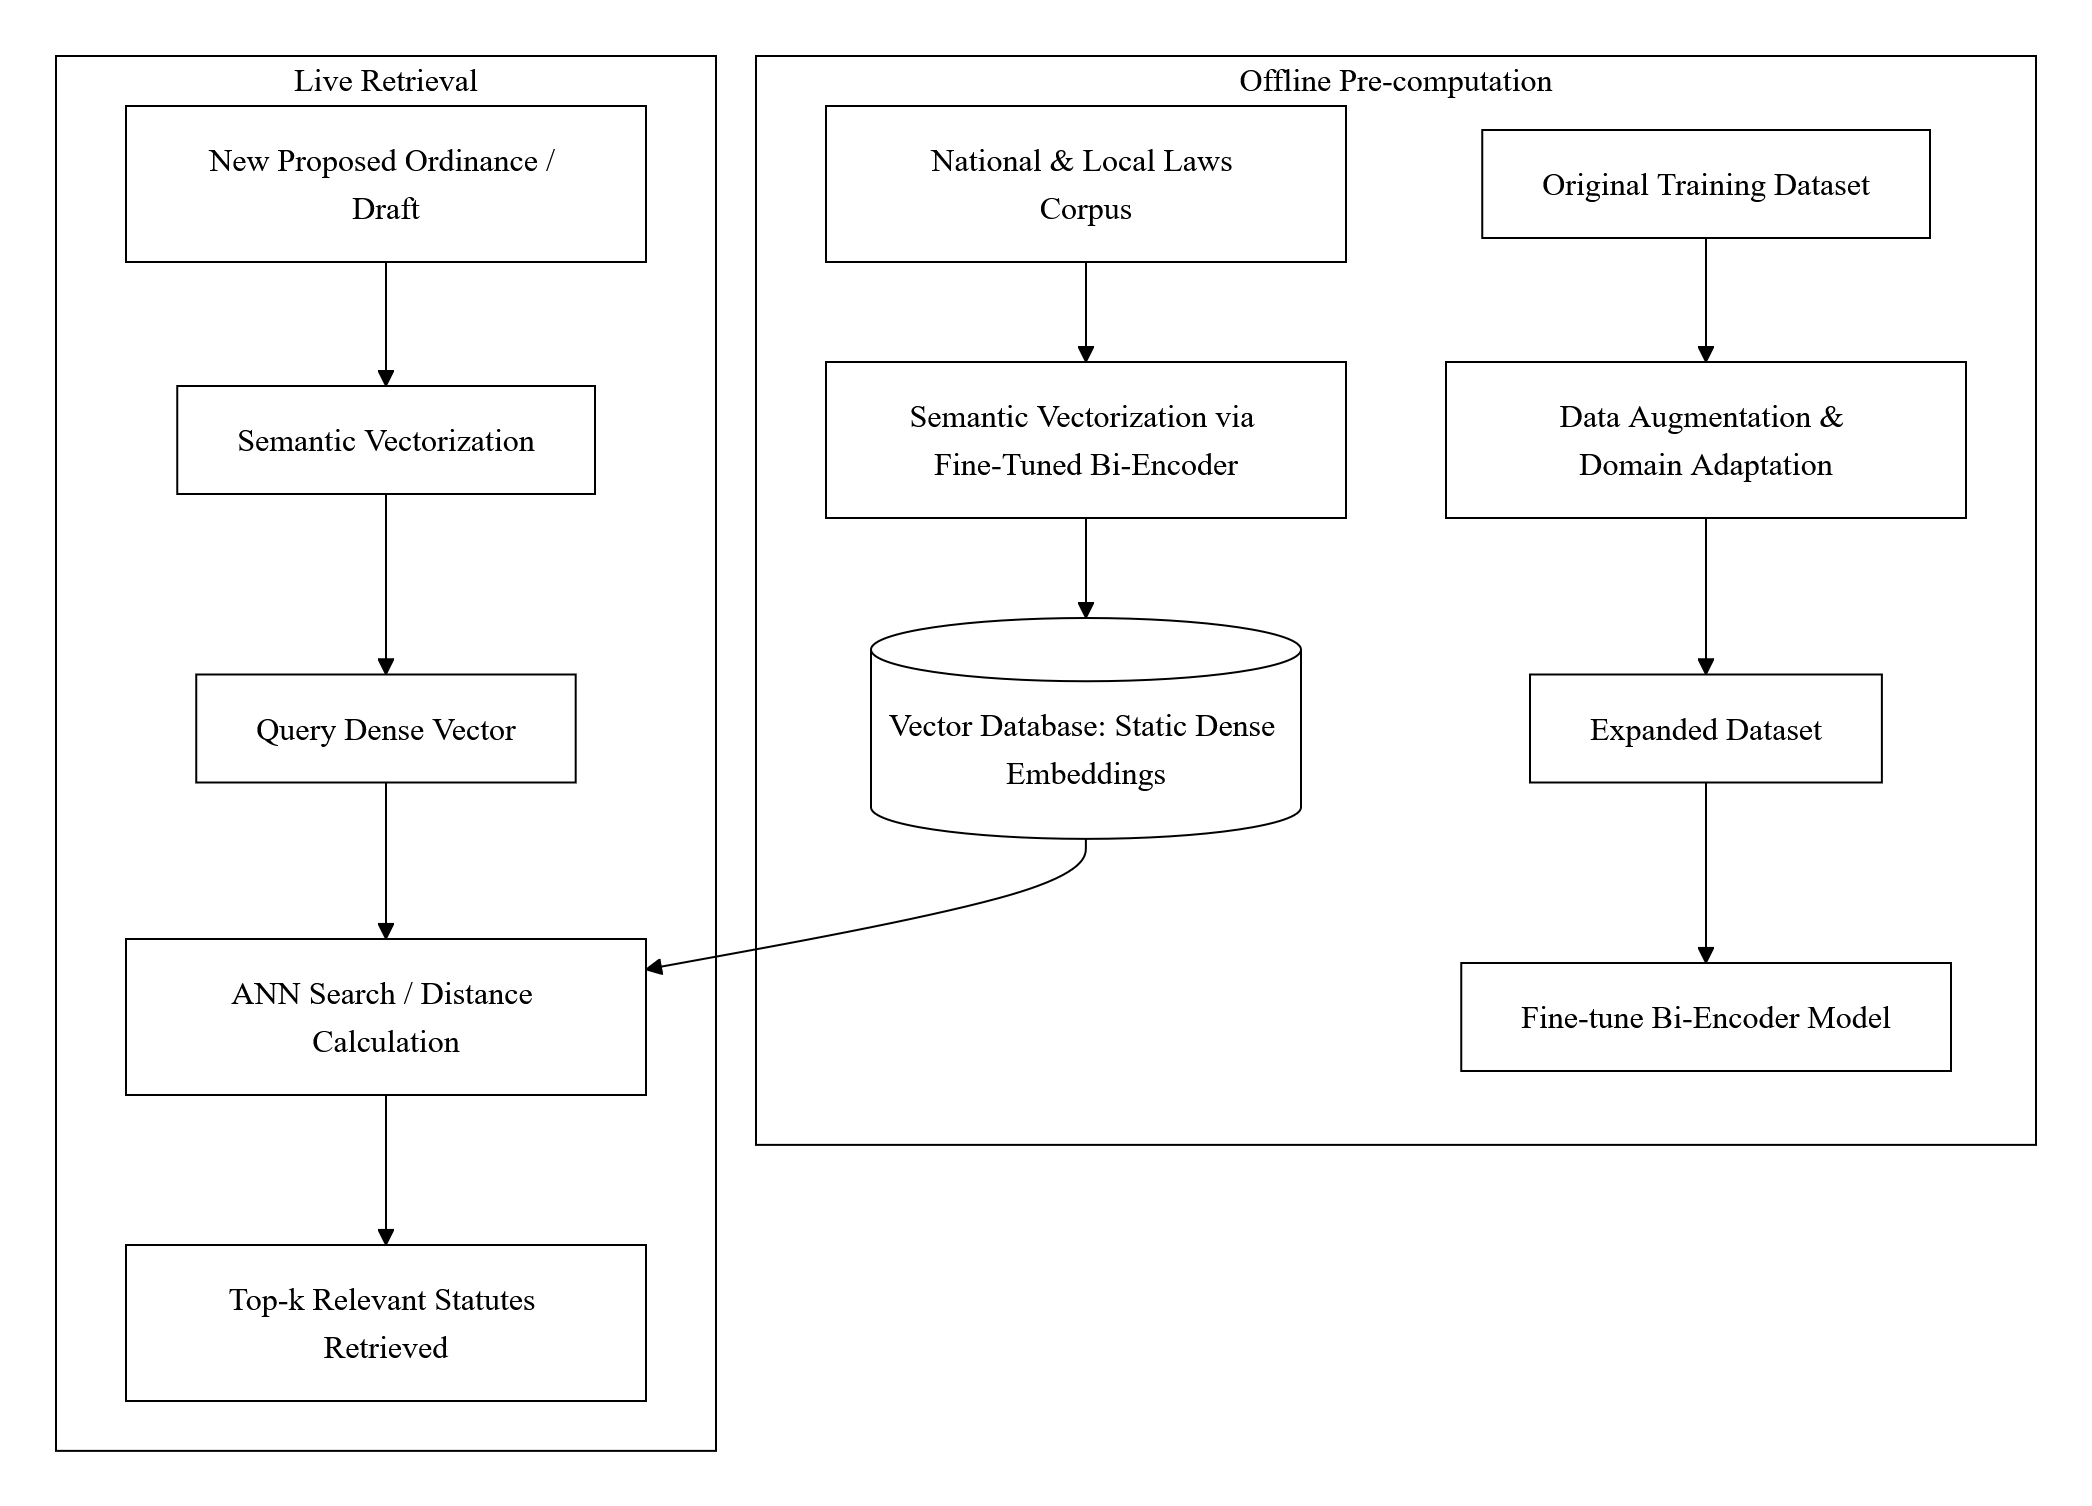
\includegraphics[width=1.0\linewidth]{figs/Phase_1_Retrieval_BW.png}
        \caption{Phase 1 - Statute Law Retrieval (Bi-Encoder Pipeline). Adapted from AIIR Lab's retrieval methodology.}
        \label{fig:phase1aiir}
    \end{figure}
    
        \begin{description}
            \item[Data Augmentation and Domain Adaptation.] By training on synthetically augmented legal datasets, dense retrieval models learn to recognize identical underlying statutory concepts regardless of whether they are expressed in archaic legal vocabulary or modern drafting syntax, substantially enhancing semantic robustness against lexical divergence.
            
            \item[Semantic Vectorization via Bi-Encoder.] The central component of Phase 1 is a Bi-Encoder architecture (such as \texttt{all-mpnet-base-v2}), which projects statutory text into a dense, continuous vector space. Unlike cross-encoders, which must process query-document pairs jointly and are computationally prohibitive across thousands of statutory enactments, bi-encoders encode queries and corpus documents independently. During contrastive fine-tuning, the embedding space is optimized such that vectors representing logically relevant statutory pairs exhibit high geometric proximity, while irrelevant pairs are separated under distance metrics such as cosine similarity.
            
            \item[Corpus Pre-computation and Vector Indexing.] To satisfy the operational requirement of querying tens of thousands of statutory documents efficiently, dense retrieval paradigms rely on offline pre-computation. Prior to query execution, the fine-tuned bi-encoder processes the statutory corpus, transforming individual statutory provisions into static, dense vector representations stored within an indexed vector database. Because corpus vectorization is decoupled from live query execution, dense retrieval scales effectively across extensive statutory archives without requiring real-time GPU re-encoding.
            
            \item[Live Query Vectorization and Proximity Scoring.] During query evaluation, the bi-encoder projects candidate draft provisions into the shared mathematical embedding space. Approximate nearest neighbor (ANN) search algorithms subsequently calculate geometric proximity (e.g., cosine similarity) between the query vector and pre-indexed statutory embeddings. Because this process computes continuous geometric distances rather than autoregressive tokens, high-throughput retrieval surfaces the top-$k$ most relevant statutory candidates in sub-second latency, providing high candidate recall to prime downstream natural language inference.
        \end{description}

    \subsection{Statute Law Retrieval by Team JNLP}
    Complementing pure bi-encoder retrieval, literature in computational law emphasizes multi-stage retrieval pipelines to balance candidate recall against ranking precision. Exemplified by Team JNLP's high-performing architecture in COLIEE benchmarks~\cite{coliee2025proceedings, goebel2026an}, this multi-stage paradigm progressively filters statutory search spaces across three structured phases: Pre-Retrieval Candidate Pruning, Model Fine-Tuning, and Result Ensembling.

    \begin{figure}[htbp]
        \centering
        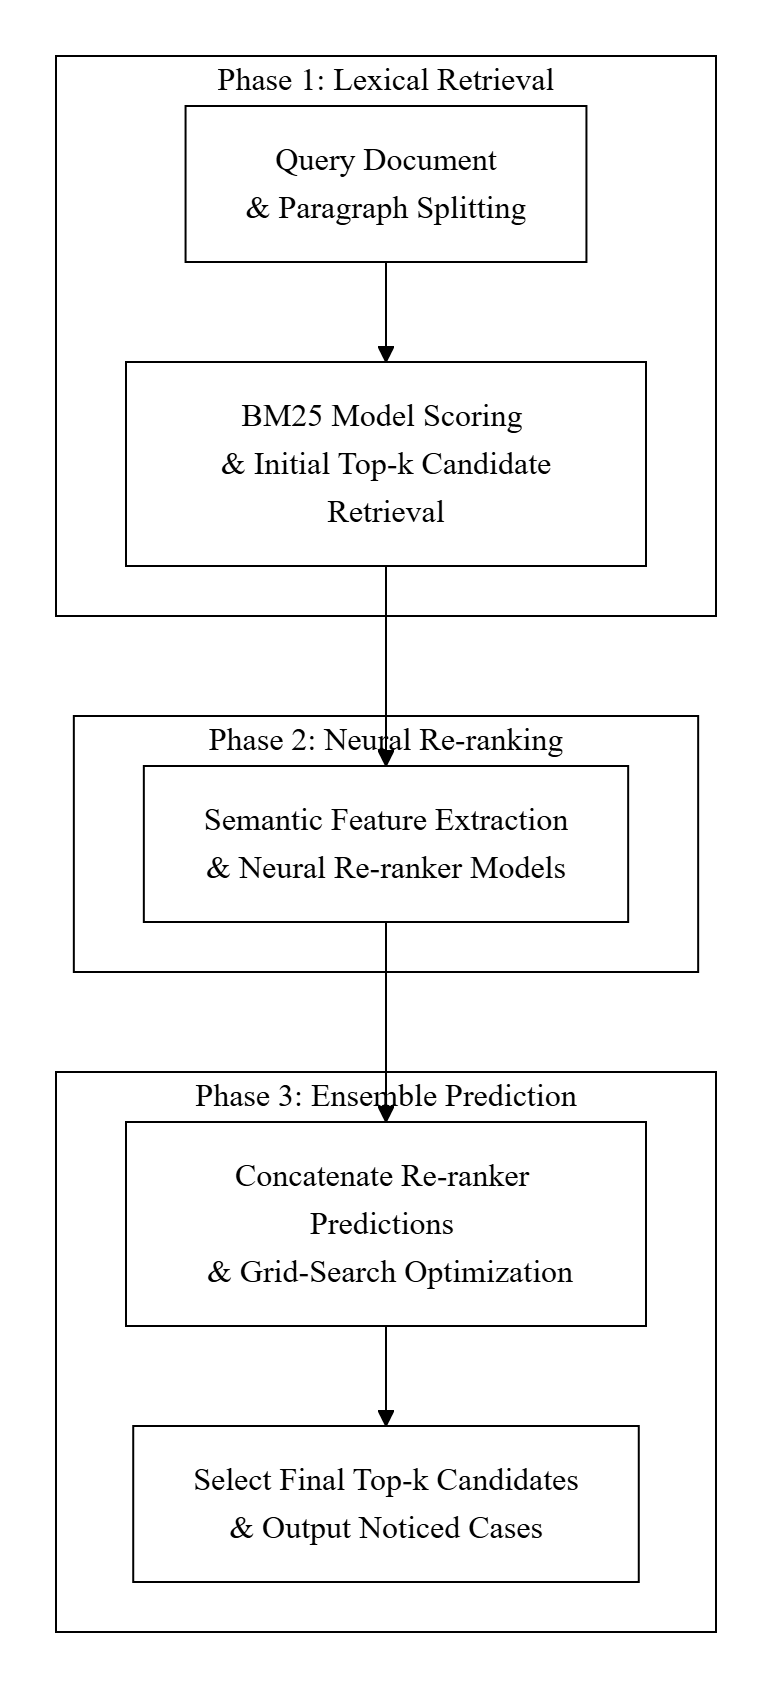
\includegraphics[width=0.6\linewidth]{figs/JNLP_Framework_BW.png}
        \caption{Phase 1 - Statute Law Retrieval (Bi-Encoder Pipeline). Adapted from JNLP's retrieval methodology.}
        \label{fig:phase1jnlp}
    \end{figure}

        \subsubsection{Pre-Retrieval}
        The primary objective of the initial phase is to drastically reduce the expansive search space while maintaining high recall across governing provisions, achieved through a multi-stage candidate pruning procedure.

            \begin{description}
                \item[Distance-Based Heuristic Filtering.] Dense embeddings for statutory queries and corpus provisions are extracted using high-capacity multilingual representations (e.g., BGE-M3). Rather than relying solely on raw cosine similarity, the methodology calculates multi-dimensional distance metrics (such as L1 distance bins), training a gradient-boosted decision tree to predict relevance and counter severe positive-negative sample imbalance.
                
                \item[Passage Re-ranking and Pruning.] The candidate pool is subsequently refined to eliminate non-relevant documents. A specialized neural passage re-ranker (such as RankLLaMA) evaluates candidate texts and prunes lower-ranked provisions, successfully narrowing the candidate set to top-ranked candidates while preserving recall.
            \end{description}

        \subsubsection{Model Fine-Tuning}
        Once the candidate space is constrained, the framework applies targeted natural language models to perform fine-grained relevance scoring.

            \begin{description}
                \item[Parameter-Efficient Model Adaptation.] Because fine-tuning large models across full parameter sets is computationally intensive, legal NLP frameworks leverage Parameter-Efficient Fine-Tuning (PEFT) techniques, such as LoRA and QLoRA. These techniques enable foundational language models to adapt to specialized statutory semantics with minimal memory overhead.
                
                \item[Class Imbalance Mitigation.] Because statutory candidate sets exhibit severe class imbalance (where only a small minority of retrieved provisions contain true preemption conflicts), sampling strategies and asymmetric loss functions are applied during training to preserve sensitivity to positive conflict signals.
            \end{description}

        \subsubsection{Result Ensemble}
        To maximize retrieval robustness and mitigate individual model variance, multi-stage retrieval pipelines aggregate relevance scores across distinct architectural paradigms.

            \begin{description}
                \item[Weighted Score Aggregation.] Rather than relying on uniform voting, relevance predictions are aggregated through weighted linear combinations of calibrated probabilities outputted by complementary lexical and neural models.

                \item[Hyperparameter Optimization.] The weighting coefficients assigned to individual scoring components are optimized via systematic hyperparameter search (e.g., Optuna), ensuring balanced contributions between lexical keyword precision and dense semantic recall.
            \end{description}

\subsection{Statute Law Textual Entailment by Team KIS}
    In the second phase of legal retrieve-then-entail architectures, the theoretical objective transitions from broad candidate discovery to fine-grained deontic reasoning. To ensure high computational throughput and deterministic classification, modern legal NLP frameworks deploy non-generative cross-encoder architectures, exemplified by the ModernBERT-based rationale extraction methodology developed by Team KIS~\cite{kadowaki2025modernbert}.

\begin{figure}[htbp]
    \centering
    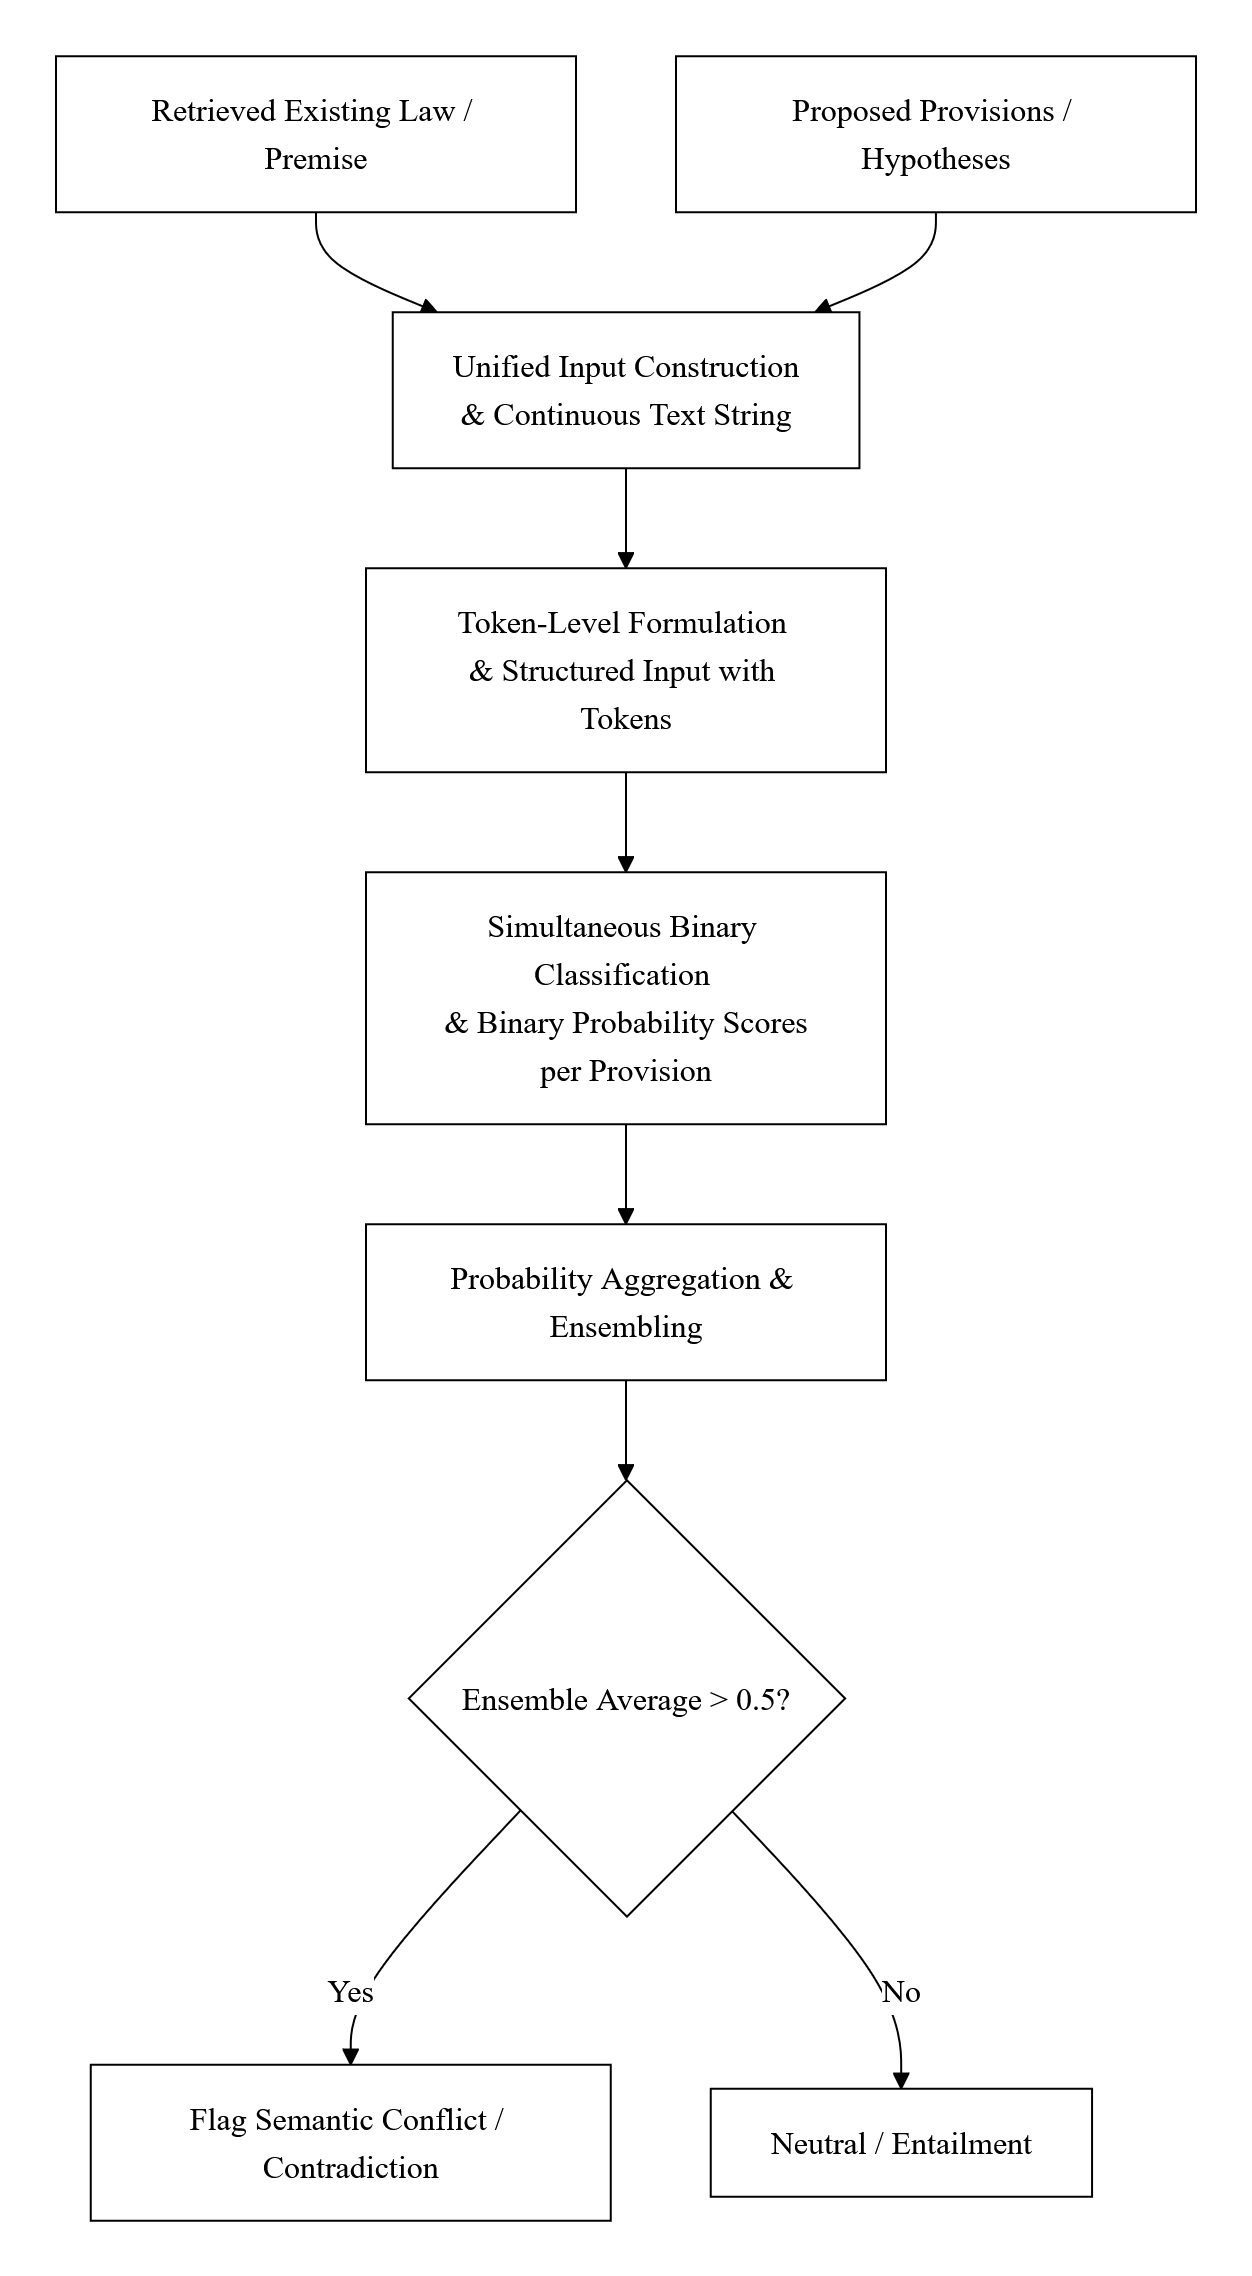
\includegraphics[width=0.7\linewidth]{figs/Phase_2_Entailment_BW.png}
    \caption{Phase 2 - Statutory Textual Entailment (NLI Pipeline). Adapted from Team KIS's ModernBERT rationale extraction methodology.}
    \label{fig:phase2}
\end{figure}
    
    This entailment framework is structured around four theoretical components:

    \begin{description}
        \item[Unified Input Construction.] While traditional transformer encoders are constrained by short sequence limits (e.g., 512 tokens), requiring aggressive document truncation, modern architectural designs support extended context windows up to 8,192 tokens. Under this formulation, retrieved statutory context (the premise) and candidate draft provisions (the hypothesis) are concatenated into a unified sequence. Strategic token boundaries clearly demarcate statutory premises from draft hypotheses.
        
        \item[Token-Level Problem Formulation.] To evaluate targeted normative conflicts within candidate provisions, the framework structures input sequences with dedicated segment tokens (e.g., \texttt{<sep>}). This formats multi-clause statutory text into an aligned representation suitable for direct cross-attention.
        
        \item[Simultaneous Multi-Target Classification.] The unified sequence is processed by an efficient bidirectional encoder. Because the architecture operates purely as a sequence classifier, it eliminates the computational latency and hallucination vulnerabilities inherent in autoregressive text generation. Instead, the model evaluates segment separation tokens to generate class probabilities, determining whether candidate provisions logically entail, contradict, or remain neutral relative to governing law.
        
        \item[Probability Calibration and Ensembling.] To maximize predictive reliability and mitigate single-model bias, the framework incorporates probability aggregation across diverse model checkpoints or hyperparameter variations. Averaged or calibrated posterior probabilities exceeding decision thresholds indicate detected normative conflict with formal statistical backing.
    \end{description}

\subsection{Theoretical Synthesis}
This synthesis integrates the foundational theoretical models reviewed throughout this chapter into a unified paradigm for ex-ante legislative conflict detection. While each individual methodology addresses an isolated phase of legal document processing, their conceptual integration establishes a principled retrieve-then-entail framework:

\begin{description}
    \item[Dense Retrieval Methodology.]
    The theoretical foundation for statutory candidate discovery draws from the dense retrieval methodology established by the \textbf{AIIR Lab}~\cite{wu2025aiir, largey2026aiirlab}. Their approach demonstrates that targeted domain augmentation mitigates OCR noise in archival legal text, while continuous semantic vectorization enables high-throughput candidate identification across large statutory collections without relying on rigid keyword indices.

    \item[Ensemble Learning Strategy.]
    To balance candidate recall against precision, the framework incorporates the multi-stage ranking principles demonstrated by \textbf{Team JNLP}~\cite{coliee2025proceedings, goebel2026an}. This methodology utilizes lexical filtering (BM25) to prune extraneous documents, followed by neural scoring and rank fusion to isolate authoritative candidate enactments on standard computing hardware.

    \item[Textual Entailment.]
    For granular deontic conflict evaluation, the framework adopts the \textbf{Team KIS framework} for textual entailment~\cite{kadowaki2025modernbert}. Their methodology formats premise-hypothesis pairs into a continuous sequence evaluated via lightweight cross-encoders, utilizing token-level separation boundaries to classify logical relationships without generative hallucination risks.

    \item[Synthesis and Benchmark Consensus.]
    Synthesizing these foundational frameworks establishes an end-to-end theoretical foundation for automated preemption auditing. The retrieval stage narrows extensive statutory search spaces down to high-probability candidate provisions, while the textual entailment stage conducts deterministic normative conflict checks. The latest findings from the COLIEE 2026 proceedings~\cite{coliee2026proceedings, ngo2026nowj} reinforce this architectural consensus, validating that pipelined retrieval and textual entailment provide the most reliable foundation for automated legal consistency analysis.
\end{description}
